\documentclass[compsoc,draftclsnofoot,onecolumn,10pt]{IEEEtran}
\usepackage[utf8]{inputenc}
\usepackage{color}
\usepackage{url}

\usepackage{pdfpages}

\usepackage{graphicx}

\usepackage{enumitem}

\usepackage[letterpaper, margin=.75in]{geometry}

\usepackage{hyperref}
\usepackage{listings}

\usepackage[dvipsnames]{xcolor}
\usepackage{pgfgantt}

\definecolor{dkgreen}{rgb}{0,0.6,0}
\definecolor{gray}{rgb}{0.5,0.5,0.5}
\definecolor{mauve}{rgb}{0.58,0,0.82}

\renewcommand{\lstlistingname}{Code Example} % a listing caption title.

\lstset{
	frame=single,
	language=C,
	columns=flexible,
	numbers=left,
	numbersep=5pt,
	numberstyle=\tiny\color{gray},
	keywordstyle=\color{blue},
	commentstyle=\color{dkgreen},
	stringstyle=\color{mauve},
	breaklines=true,
	breakatwhitespace=true,
	tabsize=4,
	captionpos=b
}

\def\name{Cierra Shawe, Daniel Stoyer, Tao Chen}

%% The following metadata will show up in the PDF properties
\hypersetup{
	colorlinks = false,
	urlcolor = black,
	pdfauthor = {\name},
	pdfkeywords = {Final Report, Winter 2017},
	pdftitle = {Final Report},
	pdfsubject = {Final Report for ARC},
	pdfpagemode = UseNone
}

\def\myversion{1.0}
\date{}
%
%\usepackage{titlesec}
%
%\usepackage{hyperref}

\parindent = 0.0 in
\parskip = 0.1 in

% \title{Capstone Final Report}
% \author{Dan Stoyer, Cierra Shawe, Tao Chen }
% \date{June 2017}

\begin{document}
\begin{titlepage}
	\title{
	Final Report\\
	ARC - Autonomous RC	\\
	\Large
	Computer Science Capstone \\
	Oregon State University\\
	Spring 2017
	}
    \author{Tao Chen, Cierra Shawe, Daniel Stoyer\\ Group 44}
	\maketitle
	\begin{center}
		\today
	\end{center}

	\thispagestyle{empty} % gets rid of the "0" page number.

\end{titlepage}

\tableofcontents

\clearpage

\section{Introduction}
Research into consumer/hobbyist, high performance RC vehicles was requested by Oregon State University via Mr. Kevin McGrath.
The project was requested to determine if it is possible to apply high-speed performance during autonomous navigation and obstacle avoidance to a modified RC car at a cost less than four thousand dollars (USD).
Autonomous RC (ARC) sought to push the boundaries of what is possible for autonomous RC vehicles.
%Not true - we didn't research this.
Our research shows that components are decreasing in cost and increasing in performance.
The cost-barrier to autonomous research is decreasing dramatically.
Our documentation and parts list provides would-be researchers a launching point to continue the work we started in ARC.
Our client was the same person who requested the project, Mr. Kevin McGrath, an instructor at Oregon State University.

\subsection{Our Team Members and Their Roles}
One of things our group is proud of, is the diversity within our group. Tao Chen is an international student from China, Cierra Shawe is one of the few female students in computer science, and Dan Stoyer is a veteran and served as a medic in the US Army.

\subsubsection*{Tao Chen}
Tao was our software and robotics expert, he worked extensively with our software package and got our car working in simulation, he was responsible for the areas of Motion Model, Path Planning, and Autonomous Algorithms (e.g. obstacle avoidance, parallel parking, etc.).\par
He will be receiving a bachelors degree in Computer Science - Computer Systems, in June of 2017. After graduation, he will be attending University of Southern California for graduate school, where he will be focusing on a masters degree in robotics.

\subsubsection*{Cierra Shawe}
Cierra was our electronics and hardware expert, she designed all the mounting hardware used to anchor the sensors to the RC car and did all the wiring/soldering. She was also responsible for the Vision Systems, Sensors, and Hardware. She will be graduating in June of 2018, with a bachelors degree in Computer Science - Applied Cyber Security. Summer and Fall term of 2017, she will be working at Rockwell Collins for an engineering co-op. She will be looking to go into a robotics field after graduation.

\subsubsection*{Daniel Stoyer}
Dan was team leader, responsible for making sure the team was on track to hit milestones and Capstone deadlines on time. He was also responsible for overseeing the areas of Image Analysis, User Interfaces, and Radio Communication. He will be graduating in December of 2017, with a bachelors degree in Computer Science - Applied Business Management, as well as a minor in business. Dan will be spending time with his newborn son (who was born during week ten of winter term) and finishing his degree, before he starts working again in tech.

\subsection{Our Clients Role in the Project}
%(i.e. supervision only, participate in development, etc.)
Our client and instructor, Kevin McGrath, provided us with general guidance and direction for the project.
Throughout the project, we met with him 30 minutes, once per week, and he would switch between the 'client hat' and the 'instructor hat' when we had questions.
As a client, when we were confused about a problem, he was able to steer us in the correct direction or give hints on what technology to look into.
He would also clarify requirements that he was expecting when we were unsure.
As an instructor, he would help clarify requirements for assignments.
Mr. McGrath also provided us with all of the hardware required for the project. When we found out something would not work, he provided us with more hardware options.

\subsection{Original Problem Statement}
(Begins on next page).

% SRS document goes here.
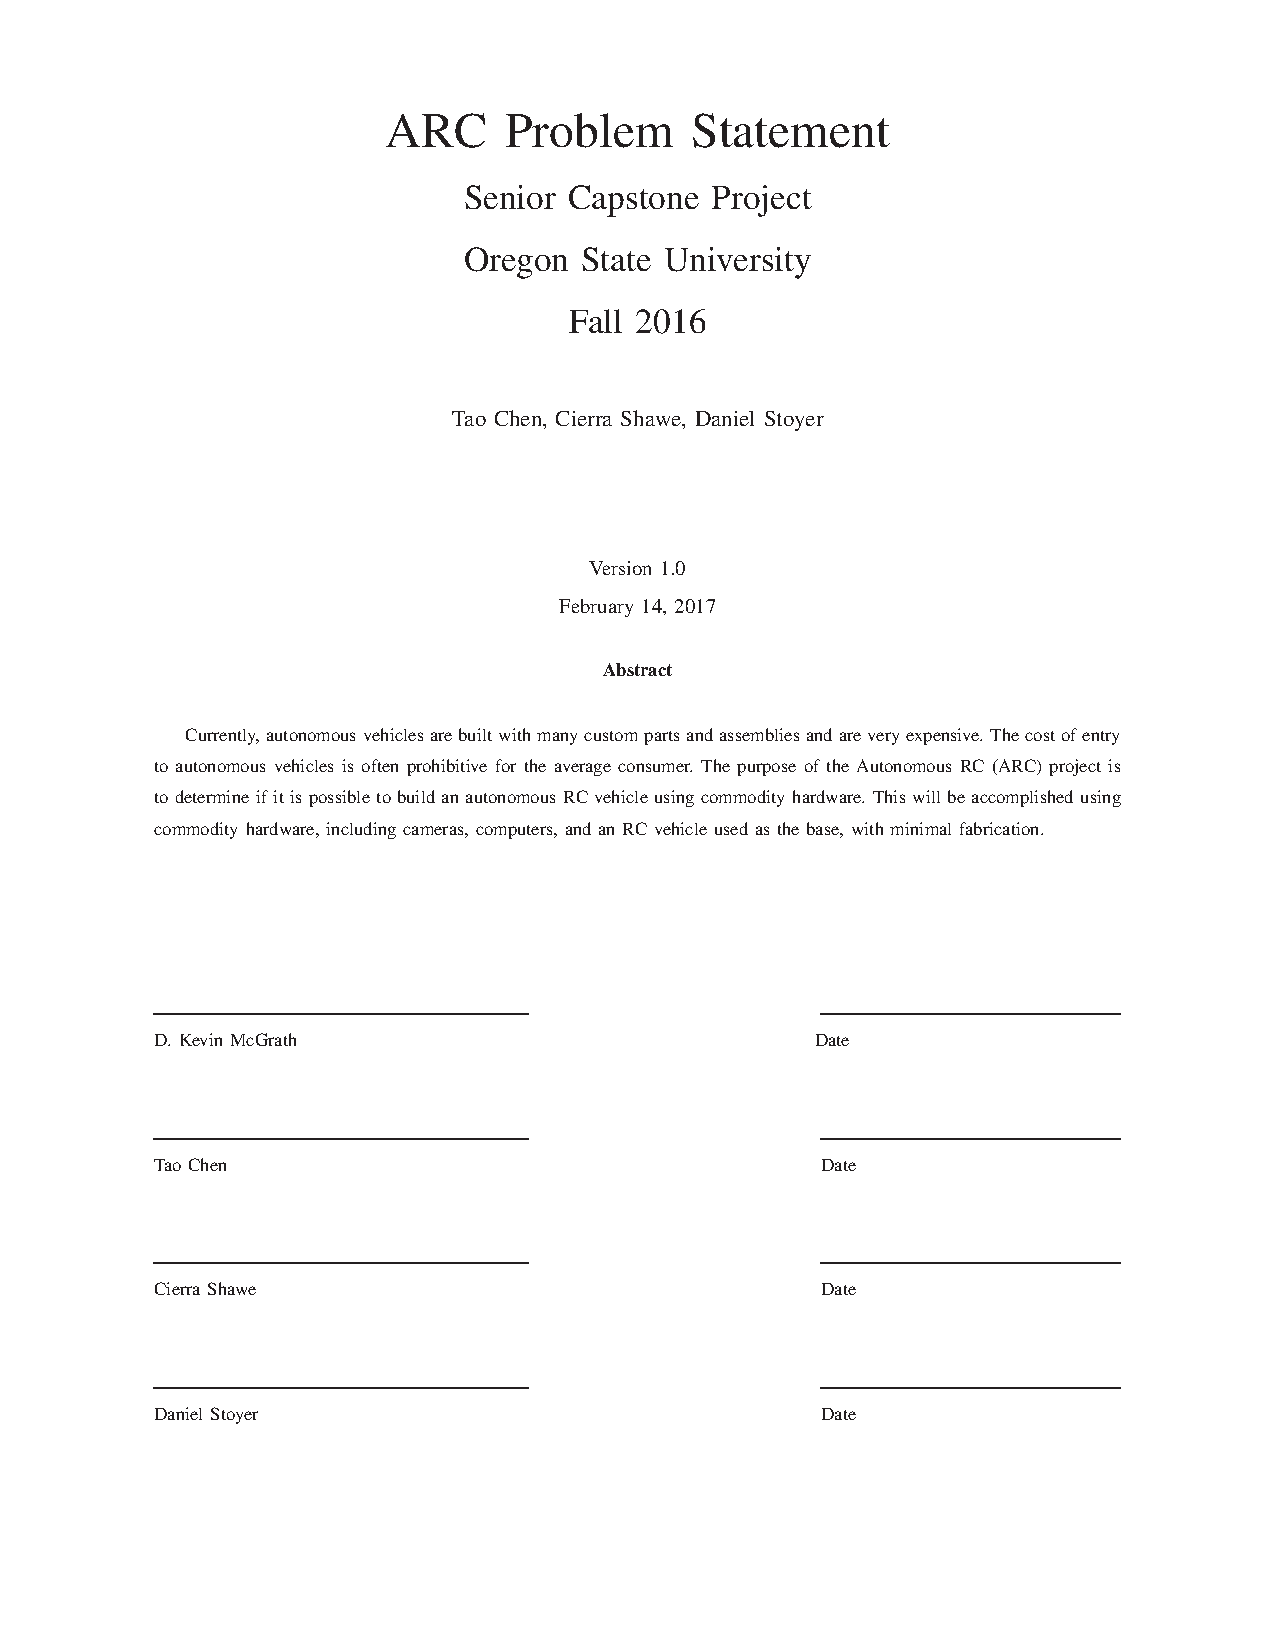
\includepdf[pages={1-3}]{problem_statement}

\clearpage
\section{Requirements Document}

\subsection{Requirements Changes}
No major or minor changes were made to the requirements document. We found that our initial assessment was accurate throughout the project and our client agreed. All results from the requirements section can be found in section 10, in "ARC Findings and Conclusions".
% Final gantt chart goes here.
\begin{figure}[h!]
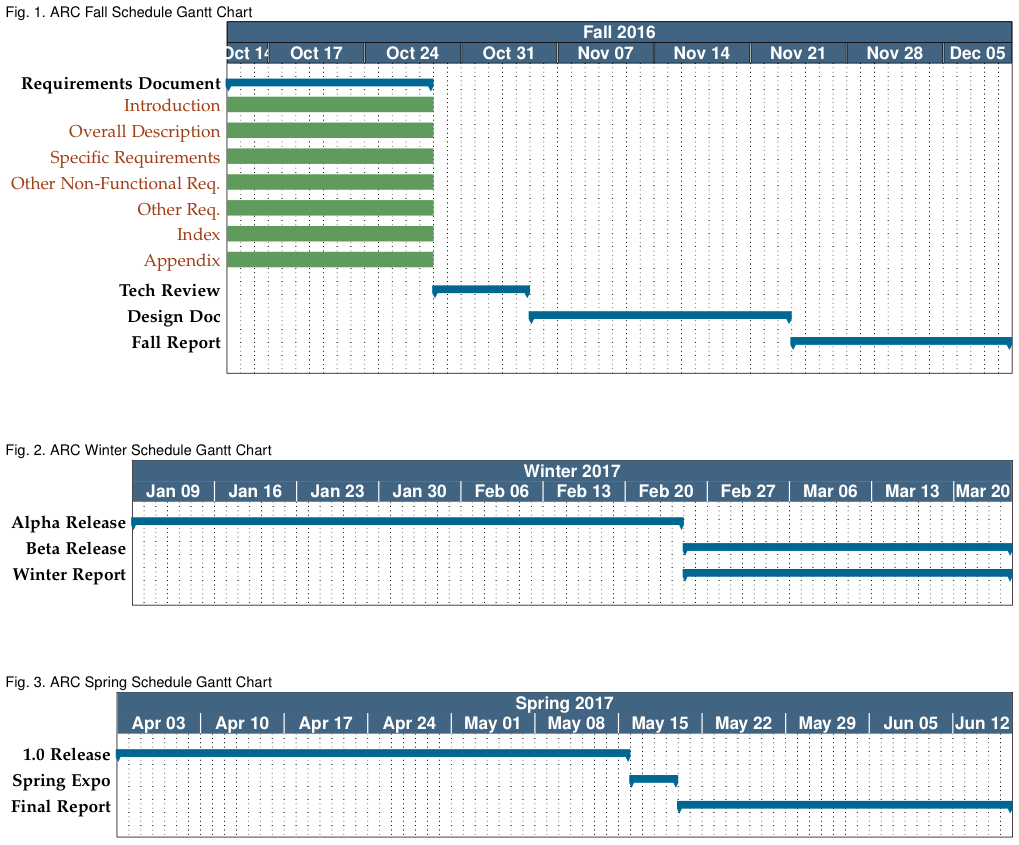
\includegraphics[scale=.5]{gantt}
\end{figure}

\subsection{Original Requirements Document}
(Begins on next page).
% SRS document goes here.

\includepdf[pages={-}]{orig_srs_document}
% Table for Client changes go here.
% \section{Document Revision History}
\begin{table}[h]
\resizebox{\textwidth}{!}{\begin{tabular}{ p{2cm}|p{1cm}|p{3cm}|p{3cm}|p{3cm}|  }

\multicolumn{5}{c}{Version History} \label{history}\\
\cline{2-2}
\multicolumn{1}{c|}{ } & Version & \multicolumn{1}{c}{ } & \multicolumn{1}{c}{ } & \multicolumn{1}{c}{ } \\
% Column format:
%<col1>&<col2>&<col3>&<col4>
%& Version & & \\
\hline
\multicolumn{1}{|c|}{Team Member}& & Cierra & Tao & Dan \\
\hline
 & v1.0 & {\tiny Initial version.} & {\tiny Initial version.} & {\tiny Initial version.} \\
\cline{2-5}
% empty first column | Cierra's changes | Tao's Changes | Dan's changes
 & v1.1 &
 % Cierra's changes
 {\tiny
 \begin{itemize}
 	\item Cierra's change \#1
 	\item Cierra's change \#2
 	\item ...
 \end{itemize}
 }
 &
 % Tao's changes
 {\tiny
  \begin{itemize}
 	\item Tao's change \#1
 	\item Tao's change \#2
 	\item ...
 \end{itemize}
 }
 &
 % Dan's changes
 {\tiny
  \begin{itemize}
 	\item Updated gantt chart with progress from Fall and Winter terms.
 \end{itemize}
 }

 \\ % End of v1.1 changes
\cline{2-5}

\end{tabular}}
\end{table}


\clearpage
\section{Design Document}
\subsection{Changes in Design}
We had to make several changes to our design throughout the life of the project.
Our vision system moved away from stereo vision for obstacle avoidance and went with LiDAR instead.
This had the benefit of simplifying our software tool-chain and network traffic load.
With our vision system using LiDAR we did not need to use OpenCV, a computer vision software library, instead we used pre-built ROS packages for the RPLiDAR and the LeddarTech LiDAR units. We were able to integrate our LiDAR units in simulation very quickly using the their pre-built packages.
Changing the vision system had a cascading effect on other parts of our design.
Since we didn't use stereo vision, our image analysis design also changed. \\
We moved away from trying to analyze images ourselves, through OpenCV or implementing our own analysis software, and used a ROS navigation stack that handled the LiDAR 2D point cloud analysis for us. An added benefit of not using stereo vision was that it greatly reduced our network overhead. The LiDAR point cloud data stream had significantly smaller packet sizes.
Our original hardware configuration included using a Raspberry Pi 2 and a PXFMini autopilot.
We abandoned both of those for a simple PWM controller to send signals to the RC car's ECS (electronic speed controller) and an Arduino to control the PWM board.
We ran into a road block with the PXFMini where we could not get the unit to receive commands.
We thought the unit to be defective, but perhaps there was some procedure we were not aware of due to our lack of experience and poor documentation for the component.
The PXFMini integrated our IMU and GPS sensor data for us, losing it meant that we had to come up with some sort of software solution to integrate the IMU and GPS data for the vehicle state estimation.
State estimation is needed for the computer to know the attitude and location of the RC vehicle in real time so that it can correct steering or speed accurately and keep the vehicle under control.
We tried to use a state estimator package from Georgia Tech's AutoRally project, but the package required specific GPS and IMU units, which we did not have.\\
Our original design called for us to use a barometer for altitude, we eliminated that option as our GPS unit already gave us altitude data. Also planned was to use ultrasonic sensors or parallel parking and redundancy in forward collision avoidance. Ultrasonic sensors were eliminated once we started using the LiDAR units. LiDAR gave us more than enough information about the world around the car and not using ultrasonic reduced the cost of the RC car overall. With two LiDAR Units we maintained redundancy regarding forward collision detection of near objects and parallel parking was achieved in simulation.\\
GT AutoRally was planned to be the base for our software platform. It appeared to handle speed control and steering nicely. The ROS navigation stack was added on after we discovered that AutoRally does not perform any sort of obstacle avoidance. We felt that trying to retro-fit such a complex platform in AutoRally with obstacle avoidance would have been time prohibitive. OpenStreetMap was an original design element intended to be used to generate way-points. We replaced OpenStreetMap with RViz, a visualization package for ROS that allowed us to set way-points and had the added benefit of consolidating sensor feedback and navigation in one application.\\
The ground station was to use an application named ArduPilot to control the vehicle remotely. ArduPilot was replaced with RViz after we discovered that RViz did everything we needed it to do making ArduPilot unnecessary.\\
Other aspects of our design staid much the same as our original design plan. Most were not tested on physical hardware, but were proven as feasible through simulation. Radio communication is one area we were not able to test in simulation and should be noted as a potential area in need of a design change.


\subsection{Original Design Document}
(Begins on next page).
    % original design document here.

\includepdf[pages={-}]{orig_arc_design_document}



\clearpage
\section{Tech Review}
\subsection{Changes in Tech}
As our research and development process matured, we discovered different ways of doing things and changed direction on some of the technology we used for the project.
We changed from stereo vision to LiDAR for depth-finding and obstacle detection.
We changed from using the PXFMini autopilot with the Raspberry Pi 3 to using a PWM controller with an Arduino to control motors and servos.
We want to use the Q Ground Control GUI to control the vehicle remotely, but had to scratch that when we abandoned the PXFMini.
We switched to using RVIZ (visualization package for ROS) for vehicle control

\subsection{Original Tech Review Document}
(Begins on next page).
% original tech review document goes here.
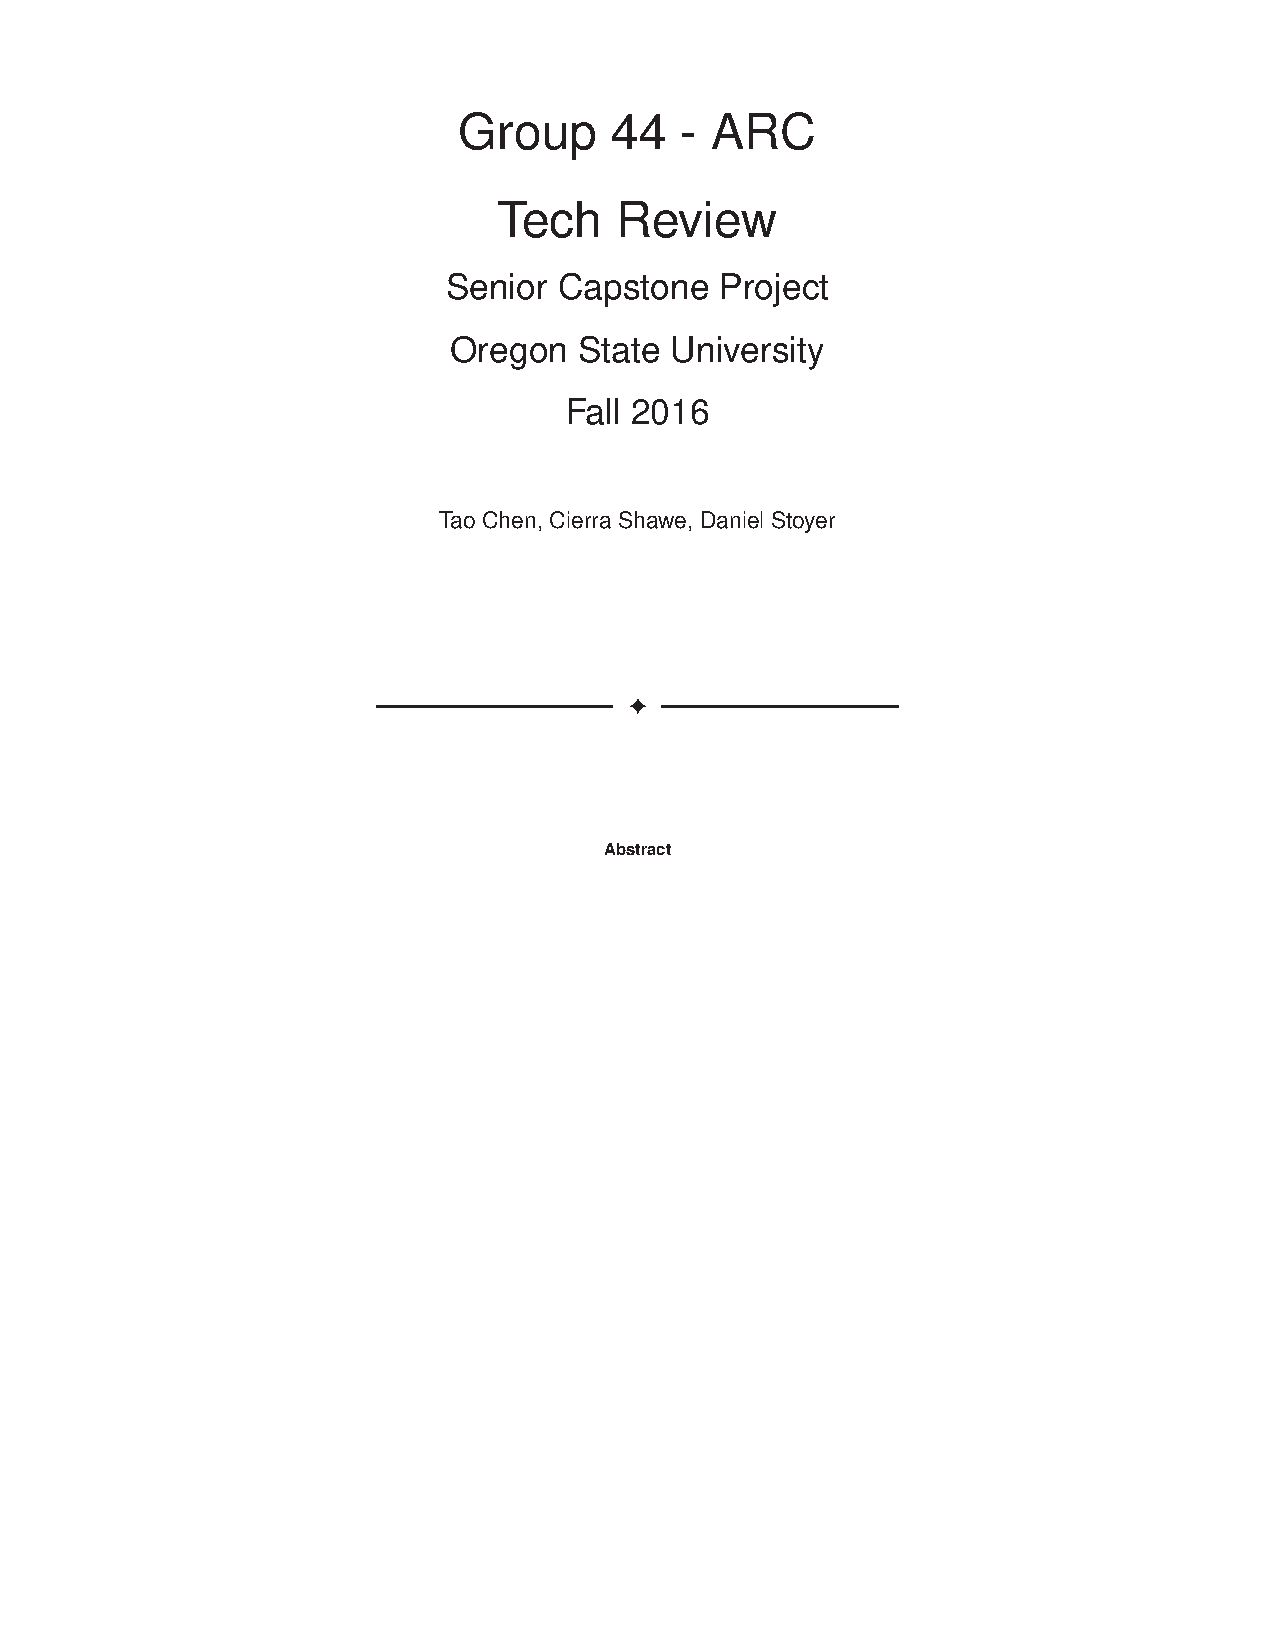
\includepdf[pages={-}]{orig_tech_review}

\clearpage
\section{Weekly Blogs}

\subsection{Cierra's Blog Entries}

\subsubsection{Fall}
\subsubsection*{Fall Week 4}
\textbf{Worked On}
\begin{itemize}
    \item This week we met with Kevin, and he asked us to add a section called "motivation" to our problem statement. Although he was mostly content with what we were saying, he wanted it to be clear from the very first paragraph, WHY this project matters, and why someone would even bother supporting it. Apparently, it went poof in his inbox, since he couldn't find it.
\end{itemize}
\textbf{Problems Encountered}
\begin{itemize}
    \item Our biggest "problem" this week, was not knowing the status of our project statement.
\end{itemize}
\textbf{Plans for next week}
\begin{itemize}
    \item Next week the goal is to get our project statement signed, on Monday in our meeting, and complete a draft of our Requirements Document.
\end{itemize}


\subsubsection*{Fall Week 5}
\textbf{Worked On}
\begin{itemize}
    \item Filling out the introduction section and other various parts of the SRS document.
    \item Overall layout of the general control flow.
\end{itemize}
\textbf{Problems Encountered}
\begin{itemize}
    \item I think our biggest problem is not having a strong understanding of specifics of our project. It's also hard to have specifics for what we will be able to do, and what we'll have, and how things will play together.
\end{itemize}
\textbf{Plans for next week}
\begin{itemize}
    \item Plans for next week include getting more specifics on the what and how portions of our requirements will work and should be within the document.
\end{itemize}


\subsubsection*{Fall Week 6}
\textbf{Worked On}
\begin{itemize}
    \item Finding out about what technology is available.
    \item Filling out sections of the SRS (hardware spec).
    \item Got an extension for the SRS.
\end{itemize}
\textbf{Problems Encountered}
\begin{itemize}
    \item The biggest problem has been finding a time where we can all get together and finish the document.
\end{itemize}
\textbf{Plans for next week}
\begin{itemize}
    \item Our main plan for next week is solidifying what our requirements are, and attempting to finish the SRS document, along with assigning "roles" or requirements of the project.
\end{itemize}


\subsubsection*{Fall Week 7}
\textbf{Worked On}
\begin{itemize}
    \item Researched different options for vision systems, and their respective advantages and disadvantages. There is a lot of research in this field, but it's hard to find tangible examples instead.
\end{itemize}
\textbf{Problems Encountered}
\begin{itemize}
    \item The biggest problem is sorting through different options, and figuring out what is reasonably implementable for our project. It's also difficult to gauge how much computing power we would need.\\
    \item Time has been a big factor for us in the past few weeks. The SRS has been very difficult without the Tech Review, as we don't know about most of the technologies that we would need. If this was a purely software based project, the SRS would have been fine because we have a general idea of what to do, versus this project has a heavy hardware focus, which makes it harder for us poor CS majors to have a crash course in basic ECE concepts. It feels as if we keep pushing deadlines, due to the overhead that this project requires in terms of material that needs to be learned. I'm not sure if I can speak for everyone, but I feel that we would all like to be able to finish our assignments in a timely manner, it just doesn't feel realistic due to all of the components required.
\end{itemize}
\textbf{Plans for next week}
\begin{itemize}
    \item The goal for next week is to finish out the tech review and finally be able to complete the SRS document. At this point, without the tech review, it doesn't seem feasible to get the SRS done without finishing the tech review first.
\end{itemize}


\subsubsection*{Fall Week 8}
\textbf{Worked On}
\begin{itemize}
    \item Worked on completing the Tech Review and updating the SRS document. Overall, the research has been slow, as documentation is a lot of information to parse through. Plus, I find research papers interesting to read, so it's hard to not get lost in all of the cool information available on different topics.
\end{itemize}
\textbf{Problems Encountered}
\begin{itemize}
    \item The biggest problem has definitely been getting the SRS done this term. We're relatively unsure of what it's supposed to look like when our entire project is based on finding if these things are even possible. The Tech Review was is also very time-consuming, since there have been a lot of unknowns within our project.
\end{itemize}
\textbf{Plans for next week}
\begin{itemize}
    \item Well, we still need to finish the SRS and start the design document. I am hesitant much will get done over Thanksgiving.
\end{itemize}


\subsubsection*{Fall Week 9}
\textbf{Worked On}
\begin{itemize}
    \item Worked on requirements in the requirements doc. Started to discuss the design document. Overall, not a lot has been completed due to the holiday.
\end{itemize}
\textbf{Problems Encountered}
\begin{itemize}
    \item Worked on requirements in the requirements doc. Started to discuss the design document. Overall, not a lot has been completed due to the holiday.
\end{itemize}
\textbf{Plans for next week}
\begin{itemize}
    \item Finish the design document and then start the end of term project write-up and video. We also still need to turn in our SRS.
\end{itemize}


\subsubsection*{Fall Week 10}
\textbf{Worked On}
\begin{itemize}
    \item Finishing SRS and design documents, basically, we want to pass this term.
\end{itemize}
\textbf{Problems Encountered}
\begin{itemize}
    \item The SRS document has been really difficult to do without the tech review and design, we really weren't able to finish the SRS. We did finally make some headway, and everything should be in by the end of the term.
\end{itemize}
\textbf{Plans for next week}
\begin{itemize}
    \item Ensure everything is turned in, and then enjoy a well needed break. Probably do some research in that time.
\end{itemize}



\subsubsection*{Fall Week 11}
\textbf{Worked On}
\begin{itemize}
    \item Finals and turned in all of our documents.
\end{itemize}
\textbf{Problems Encountered}
\begin{itemize}
    \item Not enough sleep.
\end{itemize}
\textbf{Plans for next week}
\begin{itemize}
    \item Absolutely nothing - yay break!
\end{itemize}


\subsubsection{Winter}
\subsubsection*{Winter Week 1}
\textbf{Worked On}
\begin{itemize}
    \item Tried to obtain software for our PXFmini.
    \item Worked the design for our stereo vision system. The idea is that the mount will be able to have adjustable slides in order to allow for us to test what the optimal distance for the cameras is. This first revision will be just to make sure to that the stereo vision is working correctly.
    \item We managed to find times that worked with all of our schedules, which was a big improvement over winter term. Now, we are meeting twice a week from 4pm until we are ready to finish. We also identified that Sunday afternoons are a time where we are mostly free.
\end{itemize}
\textbf{Problems Encountered}
\begin{itemize}
    \item Obtaining the software has been unsuccessful.
\end{itemize}
\textbf{Plans for next week}
\begin{itemize}
    \item My plan is to draft a CAD drawing and identify the hardware and software that we're missing. As a group, we'll start to identify what it will take to get Kevin's approval to start using the car.
\end{itemize}


\subsubsection*{Winter Week 2}
\textbf{Worked On}
\begin{itemize}
    \item Created a model to be 3D printed for our stereo-vision mount.
    \item Researched more about stereovision.
\end{itemize}
\textbf{Problems Encountered}
\begin{itemize}
    \item We are still waiting on hardware and software. This has been a huge hangup.
\end{itemize}
\textbf{Plans for next week}
\begin{itemize}
    \item Try to obtain hardware and software, and see if we can get it working together. Also, print the case for our stereo camera.
\end{itemize}


\subsubsection*{Winter Week 3}
\textbf{Worked On}
\begin{itemize}
    \item Obtained PXFmini software - however, the original image was corrupt.
    \begin{itemize}
        \item Raspberry Pi 3
        \item PXFmini software (Corrupt and working version)
        \item Motor and speed controller for testing
        \item Charger for a 3-cell LiPo battery
        \item Alligator clips to allow us to power the speed controller.
    \end{itemize}
    \item Printed camera assembly, there is a lot of room for improvement.
\end{itemize}
\textbf{Problems Encountered}
\begin{itemize}
    \item Our original PXFmini image was corrupt and we didn't have a cord to connect it to a display.
    \item The 3D print turned out well, but I've identified some things that will need to be changed: fix flanges on the assembly to either clip in, or have a better fit that accounts for different tolerances within 3D printing.
    \item I need to get a better understanding of ROS, as I'm not quite sure how to interact with it.
\end{itemize}
\textbf{Plans for next week}
\begin{itemize}
    \item My goal will be to revise our stereo mount, get it assembled (and obtain teeny, tiny screws) to keep the cameras in place.
    \item Work on getting a better understanding of ROS in order to be able to help more with the software side of the project. I've mostly been focusing on the hardware aspect of it, and I'd like to be able to help more with the software in ways other than chasing it down.
\end{itemize}


\subsubsection*{Winter Week 4}
\textbf{Worked On}
\begin{itemize}
    \item This week I worked on reassembling the camera enclosure and looking more into RTABmap.
    I had the opportunity to see a friend's project while I was in Seattle that was using a ZED and RTABmap and ROS.
    \item I also started to solder the Serial cable we needed to the IMU.
    After setting this up, I was able to get data from the IMU on a windows computer.
\end{itemize}
\textbf{Problems Encountered}
\begin{itemize}
    \item When doing the initial wiring diagram, I was going TX to RX, which should be correct; however, ultimately I needed to have TXI go to TXO and RXI go to RX0
    \item We're still waiting on more hardware, and once we have that, I can start trying to use the new LiDAR unit Kevin ordered from us.
    \item I'm worried that the rolling shutter cameras will cause problems in the future.
    \item I also need to find a ROS package for the IMU. While the Windows GUI is nice, it does not help us for integrating the IMU into our car.
\end{itemize}
\textbf{Plans for next week}
\begin{itemize}
    \item Working the ROS tutorials and attempting to calibrate the cameras. Once that is done, I would like to be able to test the camera with RTABmap.
    \item Talk to Kevin about other options for vision systems.
\end{itemize}


\subsubsection*{Winter Week 5}
\textbf{Worked On}
\begin{itemize}
    \item Attempted to get the stereo vision working through OpenCV.
    \item One of the options we are now considering is the LeddarM16 for our vision system.
    This would be paired with another LiDAR unit to provide a better range of view.
    \item I found an IMU package for ROS.
    \item I talked with Kevin, and we will try to us a LeddarM16 moving forward, to replace the stereo cameras. This will give us thousands of updates a second, in comparison to about 5. The Leddar is also really cool, because it works in direct sunlight, due to the solid state LED based system that they use.
\end{itemize}
\textbf{Problems Encountered}
\begin{itemize}
    \item I was able to view the two stereo images on the NUC, but the lag between them was almost half a second.
    Basically, that meant our stereo vision set up will not work for the project. If the two images are not able to be synced, then the computer will never be able to create a disparity map that is of any use to ROS. All in all, stereo vision will not work for our project with the current hardware.
    \item Even though I was able to find a ROS package for the IMU, which is what we need, I was not able to find any C code that would have allowed us to interface with it. Also, when I tried to watch the serial port, I was only able to see gibberish, no matter what baud rate I used.
    \item Still blocked on hardware. Even though Kevin had ordered the Leddar unit, we don't have access to the documentation and there isn't a lot about it.
\end{itemize}
\textbf{Plans for next week}
\begin{itemize}
    \item A lot of the week will probably be focused on getting the midterm together.
    \item Try to get the motors moving.
\end{itemize}


\subsubsection*{Winter Week 6}
\textbf{Worked On}
\begin{itemize}
    \item Complete the midterm report and presentation.
    \item The Leddar should be here next week.
\end{itemize}
\textbf{Problems Encountered}
\begin{itemize}
    \item We still can't talk with the NUC.
\end{itemize}
\textbf{Plans for next week}
\begin{itemize}
    \item Hopefully work with the Leddar.
\end{itemize}


\subsubsection*{Winter Week 7}
\textbf{Worked On}
\begin{itemize}
    \item Important links:
    \begin{itemize}
        \item How to enable i2c on the pi\\
        https://learn.adafruit.com/adafruits-raspberry-pi-lesson-4-gpio-setup/configuring-i2c
        \item How to use the PWM board library:\\
        https://learn.adafruit.com/adafruit-16-channel-servo-driver-with-raspberry-pi/using-the-adafruit-library
        \item Pi 3 pin layout:\\
        http://pi4j.com/pins/model-3b-rev1.html
    \end{itemize}
    \item How to move the motors and servos (as of Friday)
    \begin{itemize}
        \item Plug in the PWM usb cable to 5v power supply (ideally 2.5A).
        \item Connect Display cable
        \item Start the pi by plugging in the power supply (using ideally a 5v 2.5A/3A power supply)
        \item Navigate to ~/Adafruit\_Python\_PCA9685/examples
        \item Plug in the ESC to PWM port 1 and servos into PWM ports 2 and 3
        \item Run "sudo python esc\_test.py"
        \item Press "t" to set the esc to the top speed
        \item Plug in the battery to the esc
        \item Wait a second and then hit b to set the esc to the lower speed limit. Now you can use the arrow keys to accelerate, reverse, and turn.
        \item Hook up peripherals
    \end{itemize}
\end{itemize}
\textbf{Problems Encountered}
\begin{itemize}
    \item Just a lot of progress.
\end{itemize}
\textbf{Plans for next week}
\begin{itemize}
    \item Integrate motor control into ROS
    \item Look into GPS
\end{itemize}


\subsubsection*{Winter Week 8}
\textbf{Worked On}
\begin{itemize}
    \item Leddar! Looked into the Leddar API and Tao and I were able to get it to created a point cloud. There is a LeddarM16 ROS package, nifty!
\end{itemize}
\textbf{Problems Encountered}
\begin{itemize}
    \item There is almost no actual documentation on the Leddar.
\end{itemize}
\textbf{Plans for next week}
\begin{itemize}
    \item See about integrating both the RPLiDAR and Leddar in ROS.
\end{itemize}


\subsubsection*{Winter Week 9}
\textbf{Worked On}
\begin{itemize}
    \item We were able to get the Leddar and LiDAR working together. The Leddar really doesn't like glass, and will give wonkey readings.
\end{itemize}
\textbf{Problems Encountered}
\begin{itemize}
    \item Leddar doesn't like glass.
\end{itemize}
\textbf{Plans for next week}
\begin{itemize}
     \item Report.
\end{itemize}


\subsubsection*{Winter Week 10}
\textbf{Worked On}
\begin{itemize}
    \item Starting to get the presentation and paper together for the end of the term.
    \item Worked with Tao to get the motors turning, we are also able to control it while hard wired with a joystick. We also mapped the different outputs of the PWM controller. This was using an Arduino and a PWM controller.
\end{itemize}
\textbf{Problems Encountered}
\begin{itemize}
    \item Dan's wife had a baby. Bye bye, Dan. It's not really a problem, we just don't know when he'll be back, and will have to adjust the project accordingly for the rest of the year.
\end{itemize}
\textbf{Plans for next week}
\begin{itemize}
    \item Record and submit video.
    \item Finish and submit term report.
    \item We have finals and I leave for Seattle on Wednesday, so probably not a lot after that.
\end{itemize}


\subsubsection*{Winter Week 11}
\textbf{Worked On}
\begin{itemize}
    \item Recorded end of term video.
    \item Submitted end of paper.
\end{itemize}
\textbf{Problems Encountered}
\begin{itemize}
    \item Still no Dan. Still not a problem, but we really have no idea how this will affect us moving forward.
\end{itemize}
\textbf{Plans for next week}
\begin{itemize}
    \item Europe :D
\end{itemize}


\subsubsection{Spring}

\subsubsection*{Spring Week 1}
\textbf{Worked On}
\begin{itemize}
    \item Worked on wiring the 12v connection for the Leddar.
    \item Worked with Dan on getting the IMU and "LiDAR" sensors working in ROS.
    \item Made our schedules available to everyone so we could start planning when we will meet during the term. We also set up our meeting time with Kevin.
\end{itemize}
\textbf{Problems Encountered}
\begin{itemize}
    \item The Leddar has appeared to have died or encountered a problem with USB. We need to talk to Kevin and see what can be done to fix this.
\end{itemize}
\textbf{Plans for next week}
\begin{itemize}
    \item Try to start moving our software onto the hardware. This will allow us to test if the simulation Tao has been working on will work.
    \item We also need to make sure to register for Expo and really figure out how to implement the hardware and software solutions.
    \item Need to get radios from Kevin.
\end{itemize}


\subsubsection*{Spring Week 2}
\textbf{Worked On}
\begin{itemize}
    \item Tried various computers to see why the Leddar wasn't working.
    \item Finally created the 12v cord to power the Leddar.
    \item Dug through forums and Leddar documentation (or lack thereof) to see why our unit isn't recognized.
    \item Started to see how to wire the Leddar using rs485, and obtained the box to convert from RS485 to usb.
\end{itemize}
\textbf{Problems Encountered}
\begin{itemize}
    \item Found out the Leddar wasn't working.
    \item Found out that there is a jumper that needs to be changed for 12v operation of the Leddar, but have no idea how to change it. We still might have killed it.
\end{itemize}
\textbf{Plans for next week}
\begin{itemize}
    \item Start 3D modeling cases so we can print and cut out our soon to be sweet looking car.
    \item Help with system design and integrating software to hardware.
    \item Continue to investigate why the Leddar isn't working - follow up with support if no solution is found.
    \item Do poster.
\end{itemize}


\subsubsection*{Spring Week 3}
\textbf{Worked On}
\begin{itemize}
    \item Worked on hardware mounting. We now have a pretty box that I found in the hallway.
    \item I can now run the entire electrical system off of a LiPo battery.
    \item Performance tested the NUC. We were able to get about 1:20 minutes off of the LiPo while running the stress tests.
\end{itemize}
\textbf{Problems Encountered}
\begin{itemize}
    \item Not a lot.
\end{itemize}
\textbf{Plans for next week}
\begin{itemize}
    \item Re-design the box so it doesn't hit.
    \item Start working on GPS integration.
\end{itemize}


\subsubsection*{Spring Week 4}
\textbf{Worked On}
\begin{itemize}
    \item Obtained the new Leddar from Kevin.
    \item A lot of homework for other classes, trying to get caught up and ahead for this last push.
\end{itemize}
\textbf{Problems Encountered}
\begin{itemize}
    \item Time. Time is a problem.
\end{itemize}
\textbf{Plans for next week}
\begin{itemize}
    \item Design and print a case so we can have a snazzy car.
    \item Help with anything else I can.
\end{itemize}


\subsubsection*{Spring Week 5}
\textbf{Worked On}
\begin{itemize}
    \item Monday - Wired the pins to the GPS so we could read the data. I also worked with Dan and Tao on finally getting the GPS data. After a few hours, Tao and I were able to read the data. The problem with this, as of right now, is we are using the 3.3v power from the IMU in order to power the GPS. I will work on fixing this later, as I don't feel right using a \$180 sensor as a voltage regulator.
\end{itemize}
\textbf{Problems Encountered}
\begin{itemize}
    \item Monday - We couldn't figure out why the changes we were making to the GPS config weren't changing, and then I realized that I never soldered an RX pin to the board, so it wasn't able to read new data. To fix this, I simply held a pin in place while we made the changes, that way we had a known configuration. This also allowed us to have faster update rates.
    \item A worry with this is that the updates don't seem to be accurate enough. We will need to see if there is an orientation that both the sensor and the antenna need to be orientated.
\end{itemize}
\textbf{Plans for next week}
\begin{itemize}
    \item Submit everything we have for the code freeze...
\end{itemize}


\subsubsection*{Spring Week 6}
\textbf{Worked On}
\begin{itemize}
    \item Focused on getting all of our electrical components working. Was able to start reading GPS data from the GPS.
    \item As a group we started writing the report and progress report for the project.
\end{itemize}
\textbf{Problems Encountered}
\begin{itemize}
    \item The IMU was being used as a \$180 power source.
    \item Somehow all three of our group members misunderstood the poster submission.
    We submitted the poster and are hoping for the best.
\end{itemize}
\textbf{Plans for next week}
\begin{itemize}
    \item Start building cases. Get a new power supply.
    \item Make the box look pretty for Expo.
    \item Finish the video.
    \item Check in to make sure our poster will be done.
\end{itemize}


\subsubsection*{Spring Week 7}
\textbf{Worked On}
\begin{itemize}
    \item Printed cases for electrical components.
    \item Spray painted box and made it look cooler
    \item Finished the video, project write up draft, and midterm report.
    \item Worked with Tao on getting the servo's to be able to control the steering via the simulation.
    \item Survived Expo... Maybe not with my sanity, but definitely survived.
\end{itemize}
\textbf{Problems Encountered}
\begin{itemize}
    \item What is sleep?
    \item The ESC requires a very specific PWM signal pattern on start-up in order to program it.
    Figuring out how to do this has made it so we have been unable to get the car to be controlled via software.
    This is the last step we need to overcome in order to get the car moving on its own.
\end{itemize}
\textbf{Plans for next week}
\begin{itemize}
    \item Sleep.
    \item Sleep some more.
    \item Start working on final report.
    \item Get caught up on other classes that have been ignored (looks at technical writing)
\end{itemize}


\subsubsection*{Spring Week 8}
\textbf{If you were to redo the project from Fall term, what would you tell yourself?}\\
I would tell myself to avoid stereo-vision all together, because while it might seem like a good option, it is fairly difficult to correctly implement.
Another thing would have been to avoid using the PXFmini, as trying to get it working took up over half of a term that we could have spent implementing other features.
Finally, I would tell myself to take any time estimates, and quadruple them. Nothing will go as planned, so you need to be able to adapt to whatever is thrown your way.

\textbf{What's the biggest skill you've learned?}\\
As a whole, I have gained a lot of knowledge on how to interface hardware and software together. As an applied computer science major, I never had to take ECE classes, so things like wiring and soldering were new to me. While I had a lot of robotics experience from high school, interfacing software and hardware was always incredibly abstracted, and made as easy as possible. It was a lot different when we were given a pile of hardware and I had to start reading technical specification sheets in order to understand how it worked.

\textbf{What skills do you see yourself using in the future?}\\
I can't think of one skill that I will not use in the near future. Being able to understand technical specifications and documentation has made it so I will no longer have a hurdle of software-hardware interfaces. I have a few embedded projects I would like to pursue in the near future and this project has really broken down the walls of "I do not know where to even start."

\textbf{What did you like about the project, and what did you not?}\\
I feel incredibly fortunate to not only have had an awesome project, but an awesome team as well. It is hard not to enjoy working with a massive RC car, that has a ton of power. This project also made me really admire the autonomous vehicles that are currently being developed. \par
The only thing I did not like about the project, was the lack of actual budget. I really appreciate all of the hardware that Kevin provided us (there is a lot of it), it would have just been nice to have been able to try out some other hardware options. Some examples are a Pixhawk Mini, ZED stereo-vision camera, NVidia Jetson TX1, and more than one GPS and IMU. I can by no means complain about the hardware we were given, as we have access to some incredible things; however, I can not help but wonder if our implementation fell short of the goal because of the hardware or software. I also think that in order to determine if this is possible, or what configuration works best, would require being able to compare different pieces of hardware.

\textbf{What did you learn from your teammates?}\\


\textbf{If you were the client for this project, would you be satisfied with the work done?}\\
As a whole, yes. We started from nothing and ended up creating our own "autopilot" ROS setup, we have the car working in simulation, and we are able to turn the physical wheels on the car. Also, we were waiting on hardware until week 8 of winter term, which means a lot of our actual implementation was done within 10 weeks. If we had been able to start implementing and making significant progress in week 1 of winter, then I have no doubt that we would have been able to get the project working. \par
This project was aimed at researching the question of "is it possible," and as a whole we did determine it could be given more time.

\textbf{If your project were to be continued next year, what do you think needs to be worked on?}\\
The biggest part would be to get the motors working. Now that the platform is almost completely built, another group could focus on getting it rolling and implementing the high-speed navigation. I also think it would need at least one more GPS and IMU, along with wheel encoders, in order to give the car better odemetry. I also think it would be interesting to see a group test different hardware, and see what provides the best performance for the price.

\textbf{Speak a little about your expo experience.}\\
Expo was incredibly stressful for me, but not for the reasons most people would expect. I really do not mind talking with people, but I do have a hard time with loud areas. The group next to us had many people with very loud voices, the group next to them was blasting music most of the day, and the tents amplified the noise even more. These three things made it very overwhelming when trying to talk to people. It was also hard to not be inside the tents, as it was hot and the sun was beating down on us the entire day. One positive to our location was the tub with water and ice was right next to us.

Overall,  I had a lot of fun getting to show off our project and present in front of the advisory board. It was cool to see the overwhelmingly positive responses we were getting and the kids really liked the demo we put out with the 360 LiDAR. \par



\subsection{Tao's Blog Entries}

\subsubsection{Fall}

\subsubsection*{Fall Week 4}
\textbf{Worked On}
\begin{itemize}
  \item Worked on the problem statement performance measure section.
\end{itemize}
\textbf{Problems Encountered}\\
None.

\textbf{Plans for next week}\\
None.



\subsubsection*{Fall Week 5}
\textbf{Worked On}
\begin{itemize}
  \item Have not contributed so far.
\end{itemize}
\textbf{Problems Encountered}\\
None.

\textbf{Plans for next week}\\
None.



\subsubsection*{Fall Week 6}
\textbf{Worked On}
\begin{itemize}
  \item The SRS document.
  \item Have a better and clear view of the project.
  \item An abstract block diagram that depicts the structure of the project.
\end{itemize}
\textbf{Problems Encountered}
\begin{itemize}
  \item Still a lot of unclear/unspecified aspects of the project.
\end{itemize}
\textbf{Plans for next week}
\begin{itemize}
  \item Individual writing.
\end{itemize}


\subsubsection*{Fall Week 7}
\textbf{Worked On}
\begin{itemize}
  \item SRS document.
  \item Tasks breakdown list.
\end{itemize}
\textbf{Problems Encountered}
\begin{itemize}
  \item Still a lot of uncertainties on what hardware/interface we are using.
\end{itemize}
\textbf{Plans for next week}
\begin{itemize}
  \item Finish SRS document.
  \item Finish tech review.
\end{itemize}


\subsubsection*{Fall Week 8}
\textbf{Worked On}
\begin{itemize}
  \item Worked on the SRS document and the Tech Review. Did research on
  efficiency of specific algorithms. Since our vehicle will eventually
  run in different environments, possibly not predefined, algorithms
  must be robust as well. Thought about the project as a whole. Realized
  that we could only have a more and more thorough understanding of the
  different aspects of this project.
\end{itemize}
\textbf{Problems Encountered}
\begin{itemize}
  \item We still need more hardware. The SRS document hasn't been
  finished yet. The research we are doing currently may turn out to be
  in the wrong direction.
\end{itemize}
\textbf{Plans for next week}
\begin{itemize}
  \item Tech review and the SRS document.
\end{itemize}


\subsubsection*{Fall Week 9}
\textbf{Worked On}
\begin{itemize}
  \item Tech review and the SRS document.
\end{itemize}
\textbf{Problems Encountered}
\begin{itemize}
  \item Haven't started the design document yet.
\end{itemize}
\textbf{Plans for next week}
\begin{itemize}
  \item Start the design doc ASAP. Get more hardware in hand.
  \item We'd better have a clear view (graph/list) of we need
  to accomplish along with potential solutions.
\end{itemize}


\subsubsection*{Fall Week 10}
None.


\subsubsection*{Fall Week 11}
None.


\subsubsection{Winter}

\subsubsection*{Winter Week 1}
\textbf{Worked On}
\begin{itemize}
  \item Ros on the NUC is fully functional.
  \item Tested the LiDAR unit. It worked great.
  \item Went through some tutorials on Ros.
\end{itemize}
\textbf{Some thoughts on the project}
\begin{itemize}
  \item Start our development on the NUC and see if it is possible to
  migrate all functionalities to the Intel board at the end.
  \item Start with the LiDAR to implement obstacle avoidance.
  \item The two cameras we were given provide two separate feeds. I
  think we need two video streams in one feed such that we only need to
  dedicate one port to it and it will provide a better interface to
  interact with the images.
  \item Need to mount the two cameras on something rigid.
\end{itemize}


\subsubsection*{Winter Week 2}
\textbf{Worked On}
\begin{itemize}
  \item Ros tutorials.
\end{itemize}
\textbf{Problems Encountered}
\begin{itemize}
  \item A lot of software only supports certain versions of Ros.
\end{itemize}
\textbf{Plans for next week}
\begin{itemize}
  \item Car model on Gazebo.
\end{itemize}


\subsubsection*{Winter Week 3}
\textbf{Worked On}
\begin{itemize}
  \item More Ros tutorials. RC car model on Gazebo. Simple shape with a
  rectangular box as the chassis and four wheels.
\end{itemize}
\textbf{Problems Encountered}
\begin{itemize}
  \item Ros Indigo only works with Gazebo 2.X, which doesn't have the
  model editor built-in. So we have to code our URDF file.
\end{itemize}
\textbf{Plans for next week}
\begin{itemize}
  \item Finish the RC car model over the weekend. Make it move in
  Gazebo. Add sensors to it.
\end{itemize}


\subsubsection*{Winter Week 4}
\textbf{Worked On}
\begin{itemize}
  \item Modified the AutoRally car model.
  \item Added a LiDAR unit and a camera unit to the model.
  \item Retrieved data from the two sensors and display
  results in real time in Gazebo successfully in simulation.
  \item Migrated part of the AutoRally codes to our own package.
  \item Tried to figure out the dependencies between nodes/packages
  within the AutoRally project so that we can reuse some of them.
  \item Working on a documentation as well.
\end{itemize}
\textbf{Problems Encountered}
\begin{itemize}
  \item AutoRally is a huge project and there is a lot of physics
  involved. It might take a little bit longer than expected to go
  through all the nodes/package.
  \item The LiDAR unit worked flawlessly in Gazebo. However, the point
  cloud produced by the camera unit was rotated 90 degrees up. Worked
  on it for one day, trying to rotate it so that it actually reflects
  the reality. No luck.
\end{itemize}
\textbf{Plans for next week}
\begin{itemize}
  \item Keep on working on migrating codes. Plan to finish it by the end
  of this week. And then we can add our own stuff to it.
  \item Try to get the car moving in the simulation.
\end{itemize}


\subsubsection*{Winter Week 5}
\textit{Worked On}
\begin{itemize}
    \item Kept migrating notes while reading through the code.
    \item Tried to move the car in simulation using a joy stick.
\end{itemize}
\textbf{Problems Encountered}
\begin{itemize}
  \item Migrating code was very tedious.
  \item The platform could respond to messages from different nodes.
\end{itemize}
\textbf{Plans for next week}
\begin{itemize}
  \item Keep migrating code.
  \item Go into the AutoRally code a little deeper.
\end{itemize}



\subsubsection*{Winter Week 6}
\textit{Worked On}
\begin{itemize}
    \item Migrated notes while reading through the code.
    \item Moved the car in simulation using a joy stick.
    \item Did a little analysis on the autoRally platform. (For details, please refer to code listing in appendix)
\end{itemize}
\textbf{Problems Encountered}
\begin{itemize}
  \item The AutoRally car only follows preset waypoints.
  \item I don't know how to visualize the car in Rviz.
\end{itemize}
\textbf{Plans for next week}
\begin{itemize}
  \item Move on to generating way points.
\end{itemize}


\subsubsection*{Winter Week 7}
\textit{Worked On}
\begin{itemize}
    \item Waypoints coordinates.
    \item Thought about how to generate new waypoints based on the current environment.
    \item Looked other possible solutions for autonomous driving.
\end{itemize}
\textbf{Problems Encountered}
\begin{itemize}
  \item AutoRally uses a very weird coordinate system.
  \item Even I know the coordinate, it is still very tedious to convert a point on a normal x-y coordinate system to the one AutoRally uses.
\end{itemize}
\textbf{Plans for next week}
\begin{itemize}
  \item Tries different solutions.
\end{itemize}



\subsubsection*{Winter Week 8}
\textit{Worked On}
\begin{itemize}
    \item Worked on the navigation stack on Ros. It seems to be a promising solution we can use for our autonomous driving.
    \item The car can follow waypoints I defined manually.
\end{itemize}
\textbf{Problems Encountered}
\begin{itemize}
  \item Not much. The navigation stack seems straightforward. Making the transformation of the frames was a little confusing.
\end{itemize}
\textbf{Plans for next week}
\begin{itemize}
  \item Keep working on the navigation stack.
\end{itemize}


\subsubsection*{Winter Week 9}
\textit{Worked On}
\begin{itemize}
    \item Navigation stack. It successfully generated a path from point A to point B.
    \item I made some customized worlds with walls and obstacles using Gazebo.
    \item I tried to map the worlds I made.
\end{itemize}
\textbf{Problems Encountered}
\begin{itemize}
  \item Doing slam was a very tedious process too. I used predefined waypoints so that I did not have to do it manually. But the results were not optimal.
\end{itemize}
\textbf{Plans for next week}
\begin{itemize}
  \item Try to use an empty map instead.
\end{itemize}



\subsubsection*{Winter Week 10}
\textit{Worked On}
\begin{itemize}
    \item Empty map.
    \item Navigation stack.
\end{itemize}
\textbf{Problems Encountered}
\begin{itemize}
  \item The navigation stack has a lot of parameters. I don't understand all of them.
\end{itemize}
\textbf{Plans for next week}
\begin{itemize}
  \item Prepare for finals
\end{itemize}


\subsubsection*{Winter Week 11}
No entry.



\textbf{Note:}\par
\textit{None} indicates no blog posts were made for those weeks.\par
\textit{No entry} means blogs and notes were made but did not get posted and will
appear on later blog posts.

\subsubsection{Spring}

\subsubsection*{Spring Week 1}
\textbf{Worked On}
\begin{itemize}
  \item In the last two weeks of winter term I didn't do the whole lot
  mainly because of finals. However, I managed to get the car to follow
  paths. It turned the path planning algorithm didn't generate paths for
  the car to follow. Instead, it generates commands to drive to car. That
  made things very easy. All I did was translate the commands for the
  controller. So that's done. I have decided to use the teb\_local\_planner
  as our path planning package. I integrated it into the smart\_driving
  package and set it to work on car-like robot. According to the ros wiki
  for the car-like setup, the configuration is only experimental. Just
  something to keep in mind. It may sometimes output unpredictable behaviors.
  Since the teb\_local\_planner also does obstacle avoidance, obstacle
  avoidance was handled.
\end{itemize}

\textbf{Problems Encountered}
\begin{itemize}
  \item The steering commands oscillate a lot. The oscillation makes the
  movements of the car unnatural. We need to look deeper into the code
  to make sure the steering is smooth.
  \item Obstacle avoidance requires a lot of computing power. It requires
  so much that it's undoable on this laptop. The algorithm does obstacle
  avoidance by computing the costmap each time it sees a new objects.
  (detected by laser scans) A costmap is basically a 2D grid that describes
  the environment and helps to calculate the most efficient path. On this
  computer, a new costmap takes on average 3 seconds to compute. When
  there's no objects, the algorithm works fine on this computer. Note that
  the costmap is only updated when objects are detected. Not sure if the
  NUC can handle it. Need to find out.
  \item The software can be simplified. When I have been doing is just
  adding new nodes. I didn't consider if the nodes are actually necessary.
  It's because I didn't want to spend time on going over the AutoRally
  packages. For example, when I need to translate some data, I just make
  a node to do the task. In fact, I could have just remap the message
  name in the launch file. That will reduce a lot of overhead. It will
  possibly make the software run faster. I will make a table to figure
  out the data flow and delete all unnecessary nodes.
\end{itemize}

\textbf{Plans for next week}
\begin{itemize}
  \item Continue working on the navigation.
\end{itemize}


\subsubsection*{Spring Week 2}

\textbf{Worked On}
\begin{itemize}
  \item We decided to move away from AutoRally a little bit because it was
  too complicated. We tried ROS stage, which was a 2D simulation platform.
  It's simpler than Gazebo. We quickly got the teb\_local\_planning working
  because we already had it working with AutoRally.
\end{itemize}

\textbf{Problems Encountered}
\begin{itemize}
  \item I am not sure if stage can simulate gps and IMU. It will only simulate
  laser scan right now. If we couldn't get the IMU and gps simulated on
  stage, it is fine. We can do it directly on the car.
\end{itemize}

\textbf{Plans for next week}
\begin{itemize}
  \item Get the IMU and gps working.
\end{itemize}


\subsubsection*{Spring Week 3}
\textbf{Worked On}
\begin{itemize}
  \item Got the odometry in Stage working.
  \item Worked on the poster.
\end{itemize}
\textbf{Problems Encountered}
\begin{itemize}
  \item Stage doesn't simulate IMU.
\end{itemize}
\textbf{Plans for next week}
\begin{itemize}
  \item Keep working on Stage and the poster.
\end{itemize}


\subsubsection*{Spring Week 4}
\textbf{Worked On}
\begin{itemize}
  \item Didn't do a whole lot because I was at a point where if I couldn't
  get the IMU data I couldn't move forward in integrating the navigation
  stack. Dan and I were working on it. But we didn't make much progress.
  I had a lot homework to do. So I left it to Dan. Looks like he hasn't
  gotten it working yet.
\end{itemize}

\textbf{Problems Encountered}
\begin{itemize}
  \item The IMU driver provided by ROS outputs IMU data. However, the state
  estimator receives a constant pointer to the data. We need to find a way to
  transmit the data.
\end{itemize}

\textbf{Plans for next week}
\begin{itemize}
  \item Keep working on the IMU. If that's done. Move on to the GPS.
\end{itemize}


\subsubsection*{Spring Week 5}

\textbf{Worked On}
\begin{itemize}
  \item Worked on the GPS. The data from the GPS was not reliable.
  \item Looked for other options for state estimation, because we
  couldn't the way around the constant pointer.
  \item Found one package that seemed promising.
\end{itemize}

\textbf{Problems Encountered}
\begin{itemize}
  \item The AutoRally state estimator was a perfect package to use. But
  we didn't have the right hardware. The new package we found was intuitive
  but had a lot of parameters that needed to set up.
  \item We are still not able to set it up.
\end{itemize}

\textbf{Plans for next week}
\begin{itemize}
  \item Keep trying the new package.
  \item Start preparing for Expo (demo).
\end{itemize}


\subsubsection*{Spring Week 6}

\textbf{Worked On}
\begin{itemize}
  \item Midterm progress report.
  \item IMU and GPS.
  \item Code Freeze. Documentation.
  \item simulation.
\end{itemize}

\textbf{Problems Encountered}
\begin{itemize}
  \item Our software is very environment-dependent, meaning that it might not
  be able to run on another computer if the environment was not set up right.
  \item GPS data was still not reliable. Can't just work with the IMU.
  \item We might need wheel encoders.
\end{itemize}

\textbf{Plans for next week}
\begin{itemize}
  \item Keep preparing for the expo.
  \item Keep experimenting the new package.
\end{itemize}


\subsubsection*{Spring Week 7}

\textbf{Worked On}
\begin{itemize}
  \item Prepared the system for expo demo.
  \item Expo pitch.
  \item Expo.
\end{itemize}

\textbf{Problems Encountered}
\begin{itemize}
  \item A lot of software was installed on the laptop.
  \item Wasn't able to run the Leddar during Expo, which was kind
  of embarrassing.
\end{itemize}

\textbf{Plans for next week}
\begin{itemize}
  \item Relax.
  \item Relax more.
  \item Relax even more.
  \item Relax a little bit more.
  \item Then start working on the final write up.
\end{itemize}


\subsubsection*{Spring Week 8}

\textbf{If you were to redo the project from Fall term, what would you tell yourself?}
\begin{itemize}
  \item I would tell myself that my team would win the first prize at the end of the year.
  \item I would tell myself to get as many sensors as possible.
  \item I would tell myself this project was one of the coolest projects so do your best.
\end{itemize}

\textbf{What's the biggest skill you've learned?}
\begin{itemize}
  \item Using ROS.
  \item Communication.
\end{itemize}

\textbf{What skills do you see yourself using in the future?}
\begin{itemize}
  \item Since I will be doing robotics, I think knowing how to use ROS will greatly benefit me.
  \item I want to do research or development, which means I will most likely be working in a
  team. Good communication skill will also benefit me lot.
\end{itemize}

\textbf{What did you like about the project, and what did you not?}
\begin{itemize}
  \item I like everything about this project.
  \item I don't like the fact that we were given so many writing assignments.
\end{itemize}

\textbf{What did you learn from your teammates?}
\begin{itemize}
  \item I think my understanding of sarcasm improves a little bit.
  \item Most importantly, it's collaboration. I was working in a team with more
  than 15 people. I didn't really learn a lot from that team. A three person team
  is a good starting point. We can distribute the work load evenly and still have
  a complete picture of the project.
\end{itemize}

\textbf{If you were the client for this project, would you be satisfied with the work done?}
\begin{itemize}
  \item I will be satisfied but a little disappointed because the car can't drive itself.
\end{itemize}

\textbf{If your project were to be continued next year, what do you think needs to be working on?}
\begin{itemize}
  \item To make the project a little easier, I think we need to get another car first,
  or make one ourselves. We didn't have much information about the car we have right
  now. and that car is too much for our purposes. I want the wheels to be completely
  rigid or just with thin tires. I don't want the car to have less complicated
  suspensions and drive train.
  \item With a new customized car, we can add wheel encoders as well as arrange the
  hardware in a more elegant way. With the rigid wheels and the new suspension and
  drive train, we can gain more accuracy to the location estimate.
  \item If we have more time, we could possibly customize our own self driving package.
\end{itemize}

\textbf{Speak a little about your expo experience.}
\begin{itemize}
  \item It was very hot. And I didn't get enough free soda.
  \item We got a big table, which was nice.
  \item We were at a good location too.
  \item People seemed to enjoy our project and presentation.
\end{itemize}


\subsection{Dan's Blog Entries}

\subsubsection{Fall}
\subsubsection*{Fall Week 4}
\textbf{Worked On}
\begin{itemize}
    \item Created the problem statement tex template.
    \item The problem statement proposed solution section.
\end{itemize}
\textbf{Problems Encountered}
\begin{itemize}
    \item Not getting feedback on the revised problem statement as quickly as I would have liked.
\end{itemize}
\textbf{Plans for next week}
\begin{itemize}
    \item Create LaTeX template for the SRS.
    \item Research LaTeX Gantt charts.
    \item Start on SRS.
    \item Start on filling out a Gantt chart.
\end{itemize}


\subsubsection*{Fall Week 5}
\textbf{Worked On}
\begin{itemize}
    \item Created an SRS tex template.
    \item Did not use IEEEtran.cls because it does not format the SRS properly.
    \item I found a template online that has the proper formatting and modified it to follow the IEEE 830 documentation.
    \item https://github.com/Eisenbarth/SRS-Tex
    \item Created a new 'srs' git branch.
    \item Has a new 'srs\_template' folder with the template tex file, makefile, and supporting resources.
    \item Worked on the SRS.
    \item Filled out Software Interfaces and Communications interfaces.
    \item Found templates for LaTeX Gantt charts.
\end{itemize}
\textbf{Problems Encountered}
\begin{itemize}
    \item Trying to write a document that assumes we know what components we will need and will be using without really knowing what those things are.
\end{itemize}
\textbf{Plans for next week}
\begin{itemize}
    \item Work on SRS final draft.
    \item Work on / finish Gantt chart.
    \item Start thinking about the tech review.
\end{itemize}


\subsubsection*{Fall Week 6}
\textbf{Worked On}
\begin{itemize}
    \item Corrected our SRS tex document to use IEEEtran.cls.
    \item Corrected the heirarchy format to be numeric, instead of the default Roman numeral.
    \item Gantt chart:
    \begin{itemize}
        \item Created LaTeX document for rendering a Gantt chart:
        \item Added files and folder for Gantt chart to repo
        \item Added comments explaining how to set up groups and tasks.
        \item Filled out SRS group with sub-tasks.
        \item Created system for groups to track sub-task progress.
        \item Fixed formatting.
        \item Finished basic layout for Gantt chart
        \item Integrated gantt\_chart.tex into arc\_srs\_template.tex
    \end{itemize}
\end{itemize}
\textbf{Problems Encountered}
\begin{itemize}
    \item Getting the Gantt charts to render in LaTeX. It took around 9 hours, and it's not even close to scale-able.
\end{itemize}
\textbf{Plans for next week}
\begin{itemize}
    \item Work on finishing SRS final draft.
    \item Determine what my part of the tech review is.
    \item Work on tech review.
\end{itemize}


\subsubsection*{Fall Week 7}
\textbf{Worked On}
\begin{itemize}
    \item Tech Review: Researched image analysis software, telemetry radios, and user interfaces for drones.
    \begin{itemize}
        \item Image analysis software
        \item Found DroneKit-Python, ArduPilot, and LibrePilot.
        \item Telemetry radios
        \item Found 3DR 915 MHz Transceiver, RFD900 Radio Modem, and OpenPilot OPLink Mini Ground and Air Station 433 MHz
        \item User interfaces
        \item Found QGroundControl, DroneKit-Android, and LibrePilot.
        \item Worked on the write up for these components.
    \end{itemize}
\end{itemize}
\textbf{Problems Encountered}
\begin{itemize}
    \item The documentation for the drone software is rather vague when it comes to information on path-finding and image analysis capabilities.
    \item DroneKit documentation was somewhat confusing. At times it seemed like it was its own project, but at other times it referenced ArduPilot, making me think that DroneKit is a Python API wrapper on top of ArduPilot.
\end{itemize}
\textbf{Plans for next week}
\begin{itemize}
    \item Finish SRS document.
    \item Finish Tech Review document.
    \item Start:
    \begin{itemize}
        \item Planning the design document.
        \item Planning the progress report and presentation.
        \item Planning the poster.
    \end{itemize}
\end{itemize}


\subsubsection*{Fall Week 8}
\textbf{Worked On}
\begin{itemize}
    \item Completing tech review and additions to the srs document.
    \item Researched hardware for telemetry radios.
    \item Researched software for UI to be able to communicate with the vehicle.
    \item Researched software for image analysis for environment mapping and depth finding based off of sensor data.
\end{itemize}
\textbf{Problems Encountered}
\begin{itemize}
    \item Not too much different that other weeks: the document formats require the writer to have concrete examples and plans for where the project is going. Since this is a research project, and has not been done before, our work-flow really requires some experimentation before we can establish what is going to be used.
\end{itemize}
\textbf{Plans for next week}
\begin{itemize}
    \item Work on creating a plan that will be used in the Design Document.
    \item Create the design document.
\end{itemize}


\subsubsection*{Fall Week 9}
\textbf{Worked On}
\begin{itemize}
    \item Filled out specific requirements section of the SRS.
    \item Wrote "Radio Communications", "Image Analysis", and "User Interfaces" sections of the the tech review.
\end{itemize}
\textbf{Problems Encountered}
\begin{itemize}
    \item Having been delayed on the previous documents, we are about 1 to 1.5 weeks behind schedule. We need to finish up the srs and tech review still. This makes starting on the design document difficult, if not impossible.
\end{itemize}
\textbf{Plans for next week}
\begin{itemize}
    \item Write the design document.
\end{itemize}


\subsubsection*{Fall Week 10}

\textbf{Worked On}
\begin{itemize}
    \item Finishing the SRS and design documents.
    \item Wrote up how we will test our implementation of the ARC project.
    My part of the progress report is to synthesize my comments in these progress posts into a coherent subsection of the report.
    For the presentation, I provided summaries on power point slides, these included graphics and diagrams.
\end{itemize}
\textbf{Problems Encountered}
\begin{itemize}
    \item Our implementation for many components of ARC is currently unknown. More time is required to know exactly what specific software will be used on our project. We need to dive into the APIs used and see how compatible they are and see if we can write our own limited API (meaning simple conversions). So far we have only really had time to look into what open source resources are available at a higher level. This makes writing a detailed design document (in terms of actual code implementation) difficult. So, the design document is being written in terms of experimental plan. We have milestones that our project needs to meet. After succeeding in the first milestone, we continue to the next.
\end{itemize}
\textbf{Plans for next week}
\begin{itemize}
    \item Write up my section of the progress report.
    \item Record the progress report presentation.
\end{itemize}


\subsubsection*{Fall Week 11}
\textbf{Worked On}
\begin{itemize}
    \item Progress Report
    Created LaTeX template.
    Wrote the purpose and goals, weekly summaries for weeks 1-6.
\end{itemize}
\textbf{Problems Encountered}
\begin{itemize}
    \item It's finals week, enough said.
\end{itemize}
\textbf{Plans for next week}
\begin{itemize}
    \item It's Christmas break, but I plan to start looking into implementation, how the APIs will work.
\end{itemize}


\subsubsection{Winter}
\subsubsection*{Winter Week 1}
\textbf{Worked On}
\begin{itemize}
    \item Setting up the development environment for Linux and ROS.
    \begin{itemize}
        \item We will be using the Robotics Operating System (ROS) for communication and control of our vehicle. Linux is the operating system of choice for the ROS platform.
        \item I worked through orientation tutorials for ROS to become more familiar with the platform.
    \end{itemize}
\end{itemize}
\textbf{Problems Encountered}
\begin{itemize}
    \item No real problems encountered in week 1.
\end{itemize}
\textbf{Plans for next week}
\begin{itemize}
    \item Get Linux installed on my laptop to dual boot, also get Linux running in VMware for further testing/development capabilities.
\end{itemize}


\subsubsection*{Winter Week 2}
\textbf{Worked On}
\begin{itemize}
    \item Installed Linux to dual boot on my laptop.
    \item Got ROS running in Ubuntu 14.04 and 16.04.
    \item Got GT Autorally working in 14.04 and 16.04 in both "native" Ubuntu and in a VM.
\end{itemize}
\textbf{Problems Encountered}
\begin{itemize}
    \item My laptop died on Tuesday, so I ordered a new one and got it set up on Thursday/Friday.
\end{itemize}
\textbf{Plans for next week}
\begin{itemize}
    \item Start digging into how Autorally uses ROS and Gazebo (a simulator) to see how we can use it in our project.
    \item Look into direct computer-to-computer communication.
\end{itemize}


\subsubsection*{Winter Week 3}

\textbf{Worked On}
\begin{itemize}
    \item Continued with development environment setup.
    \item More work in ROS.
    \item Found software library for our IMU.
    \item Started looking into computer-to-computer direct communication.
\end{itemize}

\textbf{Problems Encountered}
\begin{itemize}
    \item The research I have done stated that new computer should be able to do direct ethernet communication without a crossover cable. I was not able to get the computers to communicate. I need to get a crossover cable to see if that is the issue, or if some other setting is incorrect.
    \item We received a corrupt image for the PXFMini, so we will need a new one sent to us.
    \item We were hoping we could find a ready-made computer model for our RC car for ROS or Gazebo, we have not found one as yet. This means that we might need to spend quite a bit more time building a model for simulation, if we want to go that route for development.
\end{itemize}

\textbf{Plans for next week}
\begin{itemize}
    \item Get computers talking to each other directly over ethernet.
    \item Get telemetry data from the RC to a remote computer.
    \item Get command from remote computer to RC car.
\end{itemize}


\subsubsection*{Winter Week 4}

\textbf{Worked On}
\begin{itemize}
    \item Got computers talking with each other directly over Ethernet.
    \item In Ubuntu on both systems:
    \begin{itemize}
        \item Edit wired connection
        \item set ipv4 to manual
        \item set the IP address
        \item subnet mask, and gateway
        \item The networking service may need to be started:
        \item sudo service network-manager restart
        \item Got Raspberry Pi3 talking with computers over Ethernet as well.
    \end{itemize}
    \item Worked on tutorials for ROS publishers and subscribers
    \item Got ROS publisher on computer A talking with ROS subscriber on computer B.
    \item This test is between my personal laptop and the Raspberry Pi 3.\\
        It is important that ~/.bashrc have the following lines:\\
        For computer running ROS master (this is the Raspberry Pi, and note that IP addresses are the same):\\
        export export ROS\_MASTER\_URI=http://192.168.1.2:11311\\
        export ROS\_IP=192.168.1.2\\
        For client computer (note ROS\_IP is local IP address):\\
        export ROS\_MASTER\_URI=http://192.168.1.2:11311\\
        export ROS\_IP=192.168.1.3\\
    \item Got the NUC talking to the Raspberry Pi 3 in ROS following a publisher/subscriber tutorial:\\
    http://docs.erlerobotics.com/robot\_operating\_system/ros/basic\_concepts/examples/publisher\_and\_subscribers
    \item Able to get internet working over Ethernet. This will allow us to update the Raspberry Pi3, install needed ROS packages and other library dependencies.
\end{itemize}

\textbf{Problems Encountered}
\begin{itemize}
    \item The keyboard layout on the Raspberry Pi 3 was set to UK by default.
    \item Fixed the layout permanently with: sudo raspi-config
    \item Other settings can be configured for the Pi 3 from the same config menu.
    \item WiFi is not working on the Raspberry Pi 3, internet is not working, in general.
    \item Able to get internet working over ethernet.
    \item The PXFMini did not power on.\\
    Discovered that the PXFMini cape was connected to the Raspberry Pi 3 incorrectly.\\
    After connecting correctly, the Rpi3 boots, but the PXFMini LED status lights show a code that tells us that it could not launch. This could be normal, or caused by an error. The documentation says that a vehicle selection should appear when the Rpi3 boots up, but I do not see that.
    \item Upgraded the Raspberry Pi 3 using sudo apt-get dist-upgrade and then the rpi would not boot any more.
    \begin{itemize}
        \item It turns out that the upgrade somehow wiped out the required kernel7.img needed for the OS.
        \item Copied a kernel7.img from another system image, along with other missing files, the rpi now boots, and WiFi is now working too!
    \end{itemize}
    \item Discovered that our power supply (USB power from the NUC) is under-powered for the Raspberry Pi 3, especially with the PXFMini attached. We will need to try using the DC power converter and the passthrough to the Rpi. We will need to get a voltage-meter to make sure our power is correct (need 5V, 2.5A).
\end{itemize}

\textbf{Plans for next week}
\begin{itemize}
    \item Get proper power to the Raspberry Pi 3.
    \item Get the PXFMini runnning properly.
    \item Make servos and motors run via the ROS and the PXFMini.
\end{itemize}


\subsubsection*{Winter Week 5}
\textbf{Worked On}
\begin{itemize}
    \item Got the PXFmini launched and armed with instructions for installing binaries for APMrover2.
    \item Got the Raspberry Pi 3 (RPi3) connected to the internet via ethernet using the original Erle OS image.
    \begin{itemize}
        \item Steps for connecting to internet using ethernet:\\
        In /etc/network/interfaces, uncomment the eth0 section.
        \item Steps for getting WiFi internet working with home router you will need to edit two files,
        interfaces and wpa\_supplicant.conf:
        \begin{itemize}
            \item Back up original /etc/network/interfaces file.
            \item In /etc/network/interfaces, comment out the lines for wlan0 and add the following lines
                \subitem  auto wlan0
                \subitem iface wlan0 inet dhcp
                \subitem netmask 255.255.255.0
                \subitem wpa-conf /etc/wpa\_supplicant/wpa\_supplicant.conf
            \item Back up original /etc/wpa\_supplicant/wpa\_supplicant.conf
                \subitem Edit /etc/wpa\_supplicant/wpa\_supplicant.conf:
                \subitem Comment out current network block
                \subitem Add new network={...} block containing the following lines:
                \subitem ssid="<name-of-network-ssid>"
                \subitem psk="<network-password>"
            \item Reboot the Rpi3.
        \end{itemize}
    \item I was able to publish to mavros topics and confirmed that the subscribers did get the information. So far it has not caused the actuators to fire.
    \item I was also able to confirm that the pxfmini is talking with the rpi, I can see the IMU data being transmitted and changing when I move the unit around.
    \end{itemize}
\end{itemize}
\textbf{Problems Encountered}
\begin{itemize}
    \item Continued to struggle with getting internet working using WiFi on the RPi3 and the original Erle image. This is important to get the proper software installed.
    \item I can't compile any of the code that is given in the examples because dependencies are missing... I've gotten one script to actually run, but it doesn't do anything for the pxf. and the documentation is so incomplete, it just assumes that "everything" (whatever that is) is set up and ready to go to launch the given script. And in places where it tells you to do something, it doesn't explain what is necessary for it to run, or even what the code is doing. When I try to compile a cpp file (ground\_rover.cpp) with include<ros/ros.h> the g++ compiler says it can't find the file, which means that the ros library wasn't installed into the system include directory. I can compile using an include option and point to the correct directory for the ros include libraries, but then it errors out on a different file not found in one of the included headers of ground\_rover.cpp.
    \item The instructions from erle-robotics in "first steps" show a mavros node 'raspicam\_node when running rosnode list, that node is not listed after going through their instructions. If I run rostopic list I get a similar output, but rostopics and rosnodes are two different things.
    \item Getting WiFi working for the internet breaks launching rostopics. The wifi settings must be set back to original to restore rostopic settings. -- Use erle-reset.
    \item After talking with our client, Kevin McGrath, we have determined that something is probably not set up properly, or strangery of some kind is afoot. The rpi3 and Erle PXFmini should work with the erle-image "out of the box", but it does not on our rpi3, for an as-of-yet unknown reason. Kevin and I are going to try to figure out what is going on.
    \item Well, I am now able to publish (via command line) to any of the mavros topic subscribers. I have only published to few of them, but I know how to do it now. I am also able to subscribe to topics to see what they are sending. The pxfmini is "working", in the sense that is communicating with the rpi3. I can see the IMU data, which changes when I move the pxfmini. I don't know if the numbers or correct, or even usable, but at least they are numbers...
    \item Unfortunately, nothing I have tried has gotten the actuator to move. When I arm the pxfmini, the actuator fires erratically until I send a message via mavros/rc/override, then the motor stops, but further messages do not cause the motor to do anything.\\
    At this point, I feel like I could spend the rest of the term figuring this out. Obviously that is not an option.\\
    I'm talking with Kevin about this problem. He's also having a hard time getting the pxfmini to work via software.
    \item Progress is going very slowly due to very poor documentation for the pxfmini and mavros (an api for RC communication).
\end{itemize}
\textbf{Plans for next week}
\begin{itemize}
    \item It's week 6 and the midterm report and presentation is due.
    \item Get our required One Note project environment setup and filled out.
    \item Make revisions to the documentation for my areas of focus.
    \item Make my portion of the video presentation.
\end{itemize}


\subsubsection*{Winter Week 6}

\textbf{Worked On}
\begin{itemize}
    \item Got the OneNote workbook up.
    \item Added document and presentation PDFs to OneNote.
    \item Added revision table templates to OneNote
    \item Added "template" or empty revision tables to documents (Problem Statement, Tech Review, SRS, Design).
    \item Made revisions to:
    \begin{itemize}
        \item tech review
        \item design doc
        \item Looked at srs and updated gantt chart.
        \item Created template for winter midterm report.
    \end{itemize}
\end{itemize}

\textbf{Problems Encountered}
\begin{itemize}
    \item None.
\end{itemize}

\textbf{Plans for next week}
\begin{itemize}
    \item Install QGroundControl on my system and see if we can control the pxfmini.
    \item Try to get "gtest" (a library necessary for one of the erle tutorials) installed.
    \item make a determination if we want to continue with trying to use the pxfmini autopilot or switch to a simple controller.
\end{itemize}


\subsubsection*{Winter Week 7}

\textbf{Worked On}
\begin{itemize}
    \item Got the "Teleoperating" tutorial installed. The tutorials allows control of the RC vehicle using arrow keys on the keyboard. Kevin McGrath figured out how to install it:
    \begin{itemize}
        \item mkdir -p ~/erle\_ws/src
        \item cd ~/erle\_ws/src
        \item git clone https://github.com/erlerobot/gazebo\_cpp\_examples
        \item git clone https://github.com/ros-perception/vision\_opencv
        \item git clone https://github.com/ros-perception/image\_common
        \item cd ..
        \item cd /usr/lib/arm-linux-gnueabihf/
        \item sudo ln -s libboost\_python-py34.so libboost\_python3.so
        \item sudo apt-get install libgtest-dev
        \item catkin\_make --pkg ros\_erle\_cpp\_teleoperation\_erle\_rover
    \end{itemize}

    \item The package now installs, and the keyboard changes the input to the rostopic /mavros/rc/override, but the motor does not activate.

    \item Able to set the parameter SYSID\_MYGCS, this is needed to override RC in and enable computer control of the autopilot.
    \begin{itemize}
        \item To set using \$ rosrun mavros mavparam set SYSID\_MYGCS 1, the autopilot must be launched and armed.
    \end{itemize}
    \item Able to use /mavros/rc/override to publish data to /mavros/rc/in. This is very important because it is necessary for controlling motors. The motors are still not moving, however.

    \item Installed GCS software (ArduPilot) and connected telemetry radios. Now able to see attitude of the autopilot in a gimble. But nothing else is connecting, not able to control motors at all. Cannot disarm/arm the autopilot from GCS.
\end{itemize}

\textbf{Problems Encountered}
\begin{itemize}
    \item Using the above "Teleoperation" tutorial, I am able to change the channel values for steering and throttle to /mavros/rc/in. I can see these values change on the GCS via the telemetry radios. This means that data is being sent over mavros and the telemetry radios are communicating properly. So, the problem is somewhere between /mavros/rc/in and the PXFmini. At this point we have spent almost 4 weeks trying to get the PXFmini to work. This was supposed to work "out of the box". We will move on to a different autopilot.
\end{itemize}

\textbf{Plans for next week}
\begin{itemize}
    \item Work out the kinks while installing AutoRally.
\end{itemize}

\subsubsection*{Winter Week 8}
\textbf{Worked On}
\begin{itemize}
    \item Went through uninstalling and reinstalling Autorally.
    \item The autorally softare package has a few different parts to it and odd/obscure errors can occur during installation. My goal was to find errors that arise and document how to fix/correct them so that users will have a better installation experience and get the system up and running faster.

    \item Found the following error:
%FIXME line wrapping
\begin{verbatim}
CMake Error at autorally/autorally\_control/CMakeLists.txt:19 (find_package): By not providing "FindEigen3.cmake" in CMAKE_MODULE_PATH this project has asked CMake to find a package configuration file provided by "Eigen3", but CMake did not find one.

Could not find a package configuration file provided by "Eigen3" with any of the following names:

Eigen3Config.cmake
eigen3-config.cmake

Add the installation prefix of "Eigen3" to CMAKE_PREFIX_PATH or set "Eigen3_DIR" to a directory containing one of the above files. If "Eigen3" provides a separate development package or SDK, be sure it has been installed.
\end{verbatim}

\item This was resolved by changing the calling CMakeLists.txt file:\\
Original: find\_package(Eigen3 REQUIRED)\\
Changed to:\\
find\_package(PkgConfig)\\
pkg\_search\_module(Eigen3 REQUIRED eigen3)\\

\item I was able to reproduce the above error and verify the above fix worked consistently. I have not been able to test this on other systems.

\item Worked through the uninstall process and identified where files were install to, this mostly had to do with GTSAM installation. Autorally itself is fairly localized and doesn't install any libraries to /usr/..

\item I have a fairly solid grasp of the uninstall/reinstall process for autorally, which means that as we move forward with integrating our own software we will be able to provide a more smooth experience for other users through documentation, and perhaps automation of the installation process.

\item Still not sure if the Eigen3 error is something that will occur on a first-time install. I don't recall seeing the error before.

\end{itemize}

\textbf{Problems Encountered}
\begin{itemize}
    \item It took a few days to figure out what all needed to be cleaned out of the system to be able to reinstall the software. Then it took another day or two to figure out how to resolve installation errors that we hadn't seen before.
\end{itemize}

\textbf{Plans for next week}
\begin{itemize}
    \item         \item Get autorally installed with the new files Tao is working on.
    \item Get Telemetry radios working without the pxfmini...
\end{itemize}

\subsubsection*{Winter Week 9}
\textbf{Worked On}
\begin{itemize}
    \item Integrating Tao's implementation in to the installation process.
    \item Able to launch rviz using a custom configuration file. This allows us to load a specific configuration on different computers which will eliminate the need for tedious setup of the rviz environment.
\end{itemize}

\textbf{Problems Encountered}
\begin{itemize}
    \item None this week.
\end{itemize}

\textbf{Plans for next week}
\begin{itemize}
    \item Continue with building our installation process.
\end{itemize}

\subsubsection*{Winter Week 10}
\textbf{Worked On}
\begin{itemize}
    \item None
\end{itemize}

\textbf{Problems Encountered}
\begin{itemize}
    \item My wife had a pregnancy-related emergency and our son was born via emergency c-section.
\end{itemize}

\textbf{Plans for next week}
\begin{itemize}
    \item None.
\end{itemize}


\subsubsection*{Winter Week 11}
\textbf{Worked On}
\begin{itemize}
    \item None.
\end{itemize}

\textbf{Problems Encountered}
\begin{itemize}
    \item I was in the NICU in Eugene.
\end{itemize}

\textbf{Plans for next week}
\begin{itemize}
    \item None -- Spring Break
\end{itemize}


\subsubsection*{Spring Week 1}
\textbf{Worked On}
\begin{itemize}
    \item Talked through the complexity of AutoRally with Tao and Cierra. We determined that AutoRally is too complex to try to integrate into our project in the time-frame we have left. We decided to drop AutoRally and focus solely on ROS for the navigation stack.
\end{itemize}

\textbf{Problems Encountered}
\begin{itemize}
    \item The physical USB port on one of your telemetry radios broke. We cannot do radio communication until it is fixed.
\end{itemize}

\textbf{Plans for next week}
\begin{itemize}
    \item Get the IMU, LiDAR, Leddar, and GPS drivers installed on the NUC.
\end{itemize}


\subsubsection*{Spring Week 2}
\textbf{Worked On}
\begin{itemize}
    \item Installed the IMU and LiDAR drivers on the NUC.
    \item Got rostopics for the IMU and LiDAR publishing data and able to visualize the data in RViz.
    \item Worked with Tao on figuring out how to get another simulation (Stage) working with our hardware packages.
\end{itemize}

\textbf{Problems Encountered}
\begin{itemize}
    \item The Leddar unit is not being recognized in Windows or Linux via USB. It was working earlier, but isn't now. We will try the RS485 interface to see if the Leddar unit is bad, or just the USB interface.
\end{itemize}

\textbf{Plans for next week}
\begin{itemize}
    \item Integrate IMU and GPS.
    \item Get simulation stable using GPS to smooth out the IMU calculations.
    \item Refine hardware mounting on the car
\end{itemize}

\subsubsection*{Spring Week 3}

\textbf{Worked On}
\begin{itemize}
    \item Edited the outcomes and findings for the poster.
    \item Continued to try to get IMU and GPS data converted into something the AutoRally state estimator will accept.
\end{itemize}

\textbf{Problems Encountered}
\begin{itemize}
    \item Still having no luck converting the data we need.
\end{itemize}

\textbf{Plans for next week}
\begin{itemize}
    \item Help Tao with the simulations and Cierra with the hardware mounting.
\end{itemize}


\subsubsection*{Spring Week 4}

\textbf{Worked On}
\begin{itemize}
    \item Attempting to convert our ROS-published IMU data to something that IMUGPSestimator can use. IMUGPSestimator is from GT AutoRally, we need it to integrate our GPS and IMU data to determine the position of the car in the world.
\end{itemize}

\textbf{Problems Encountered}
\begin{itemize}
    \item We need the IMU and gps data to accurately track the position of our car in the world. Integrating that data is not trivial. This is absolutely required to do any autonomous navigation in the real world. It turns out that this very problem is what was really helpful in having an autopilot. The autopilot does all this integration for you. Without the autopilot we have to come up with an integration and interpretation solution on our own.
\item We do not have time to develop our own software to integrate GPS and IMU data to accurately track the position of our car in the world.
\begin{itemize}
    \item We are trying to use the estimator from GT AutoRally to integrate GPS and IMU data. However, IMUGPSestimator subscribes to a different data type (IMUConstPtr) than the data type published by by our IMU (IMU data type).
    \item We are trying to resolve this difference by converting IMU to IMUConstPtr. This has proven very challenging. There is no documentation on what IMUConstPtr actually is. The definition shows us that it's super type is shared\_ptr from the Boost library.
    \item shared\_ptr seems to be a generic type used to track pointer usage and garbage collect automatically when the pointer is no longer used. It does not seem to be relevant to our need to convert from IMU to IMUConstPtr.
\end{itemize}

\item So far, we have not been able to convert the data.
\end{itemize}

\textbf{Plans for next week}
\begin{itemize}
    \item Do as much as we can to get our software running the car.
    \item Get the poster more-or-less finalized and approved by our client.
    \item Get all the code we have been working on/with uploaded to our Github repo.
    \item Submit our poster for print before May 1.
\end{itemize}


\subsubsection*{Spring Week 5}
\textbf{Worked On}
\begin{itemize}
    \item Continued researching how to convert our IMU data into the constant pointer data structure that AutoRally wants.
    \item Reviewed the poster put together by Cierra and Tao while I've been caring for my wife and newborn son.
    \item Worked with Tao on finding different simulations to possibly use during Expo.
\end{itemize}

\textbf{Problems Encountered}
\begin{itemize}
    \item Adjusting to a newborn baby is rough!
    \item Getting accurate state estimation for the vehicle is proving problematic.
    \item We found out that we misunderstood poster submission requirements. We did not submit the printing job to Printing Media Services within the allotted time-frame for Engineering Expo posters.
\end{itemize}

\textbf{Plans for next week}
\begin{itemize}
    \item Continue to hack away at getting sensor data integrated and experiment with our navigation stack in simulation.
    \item Work on our mid-term submission requirements.
    \begin{itemize}
        \item Written progress report
        \item Progress report video
        \item Expo pitch
        \item Final project write up rough draft.
    \end{itemize}
    \item Practice project presentation for the advisory board.
\end{itemize}


\subsubsection*{Spring Week 6}
\textbf{Worked On}
\begin{itemize}
    \item Worked with Tao testing a simulation package called Stage. It is very light-weight and, used with RVIZ, it allows use to control and environment and display our car much more simply than Gazebo allows. We will likely use this combination, Stage with RVIZ, to present at Expo.
    \item Wrote my section of the mid-term progress report.
    \item Tao, Cierra, and I recorded the mid-term progress video.
    \item Wrote up my section of the write-up rough draft, which was very similar to the progress report.
    \item We worked on our Expo pitch and project presentation. I am doing the intro, Tao is talking about what we did, and Cierra is wrapping things up in the conclusion.
\end{itemize}

\textbf{Problems Encountered}
\begin{itemize}
    \item We are still struggling with getting the data from the navigation stack to be usable on actual hardware. The main problem is that the simulation is using "perfect" data for the sensors, in real life the sensor give somewhat inaccurate data. This can be countered by adding redundant sensors to increase noise, which smooths out the data, and/or add an odometry encoder to the car to track distance traveled which, added to the data from the sensors, will give the software a more accurate estimation of the state of the car.
\end{itemize}

\textbf{Plans for next week}
\begin{itemize}
    \item Last minute work on expo presentation.
    \item Build stand for the car.
    \item Give project presentation to the advisory board.
    \item Do Expo.
\end{itemize}


\subsubsection*{Spring Week 7}
\textbf{Worked On}
\begin{itemize}
    \item Built stand for the car.
    \begin{itemize}
        \item Designed base and legs to raise and support the vehicle off the ground.
        \item Painted the stand with a gloss finish coat.
    \end{itemize}
    \item Gave project presentation to the advisory board.
    \item Presented our project at Expo.
\end{itemize}

\textbf{Problems Encountered}
\begin{itemize}
    \item No major problems encountered this week.
\end{itemize}

\textbf{Plans for next week}
\begin{itemize}
    \item Continue to try to implement functionality for hardware.
    \item Build out some of the interfaces to allow for future projects to implement the hardware.
    \item Continue working on the instructions/documentation so that future projects will be able to get to the point we are at very quickly and go from there.
    \item Work on the Project Write Up, add more detail and refine the findings and conclusion sections.
\end{itemize}


\subsubsection*{Spring Week 8}

\textit{If you were to redo the project from Fall term, what would you tell yourself?}
\begin{itemize}
    \item Identify critical points of failure. Things that could possibly set us back significantly if they were to fail.
    \item Test those points early, if possible.
    \item Be more proactive about getting help for problems. Don't struggle with a problem for more than a few days before getting help.
\end{itemize}

\textit{What's the biggest skill you've learned?}
I learned about the Robotics Operating System (ROS), a general purpose, open source platform for robotics communication and operation. ROS provides a wide range of libraries for communication and control of many kinds of robots, from mechanical arms to rovers, like the car we worked on during Capstone. This project was complicated enough and covered a long enough period of time that I was able to research ROS in depth. I went through beginner tutorials to understand the basics of how ROS works and then applied some of the concepts from the tutorials to our specific needs in our project. I was able to go through a fairly complete learning cycle to become comfortable with how ROS works. In addition, I had no prior experience with autonomous vehicles, this project gave me exposure to the world of autonomy and gave me a greater appreciation and understanding of what is involved for vehicles to operate autonomously.

\textit{What skills do you see yourself using in the future?}
\begin{itemize}
    \item Computer Science is about solving problems (or trying to...), this project required us to answer the question, "Is high performance autonomous navigation possible on inexpensive hardware?" We had to identify the problem we were trying to solve, research possible techniques/approaches for solving the problem, test our solutions, make adjustments and try again, communicate with a client and conform to requirements, work as a team for a "long" period of time, then arrive at a conclusion and present our findings and conclusion.
    \item These experiences help develop/refine a wide range of skills, both technical and relational, that apply directly to the CS field and life in general.
\end{itemize}

\textit{What did you like about the project, and what did you not?}
\begin{itemize}
    \item I liked my client and my team. Cierra and Tao were great teammates and always positive, eager to work on the project. Kevin was a great client, giving us pointers and keeping expectations within reason.
    \item I liked that we had several terms to work on the project, this allowed us to do something fairly significant and complex, versus only having one term as would be the case with a normal course.
    \item I liked the project itself, learning about autonomous vehicles and the current state of the hobbyist-level in this field was very interesting and it was fun to try to get our car working.
    \item I was not a fan of having to do so many "Progress Report" videos. They were quite time-consuming and a little frustrating. Each progress report took around a week to put together, that's about 4 weeks taken from Fall and Winter terms. I realize that accountability needs to be maintained, perhaps the written report would suffice? It seemed like our weekly meetings with our TA were like a running version of the video.
    \item I did not really like the "Wired" article. I get that the point was to practice our expo pitch and interact with others, but grading us on the formatting and style of writing was a bit much.
\end{itemize}

\textit{What did you learn from your teammates?}
I learned from them how to have fun with the process. I think at the beginning of the project my demeanor was too serious. Their enthusiasm and general positivism helped me lighten up and have more fun (I don't know if they would agree, haha). I learned more about electronics from Cierra and more about software simulations from Tao.


\textit{If you were the client for this project, would you be satisfied with the work done?}
I think I would be satisfied. Our objective was to determine if it's possible to make a high performance autonomous RC car with inexpensive hardware and open source software. We put more than sufficient work to come a informed conclusion on the matter.


\textit{If your project were to be continued next year, what do you think needs to be working on?}
A team would need to take our hardware and software platform and work on creating a state estimator with the sensors and data we are using. The state estimator is need to keep the car in control during autonomous operation.


\textit{Speak a little about your expo experience.}
Expo was a fun experience for me, overall. We gave a presentation of our project to the industry advisory board and then talked with attendees during the event. It was fun explaining what we did and why we did it. I talked to quite a few kids and it was really fun seeing them interested in the project and answering their questions.


\clearpage
\section{Project Poster}
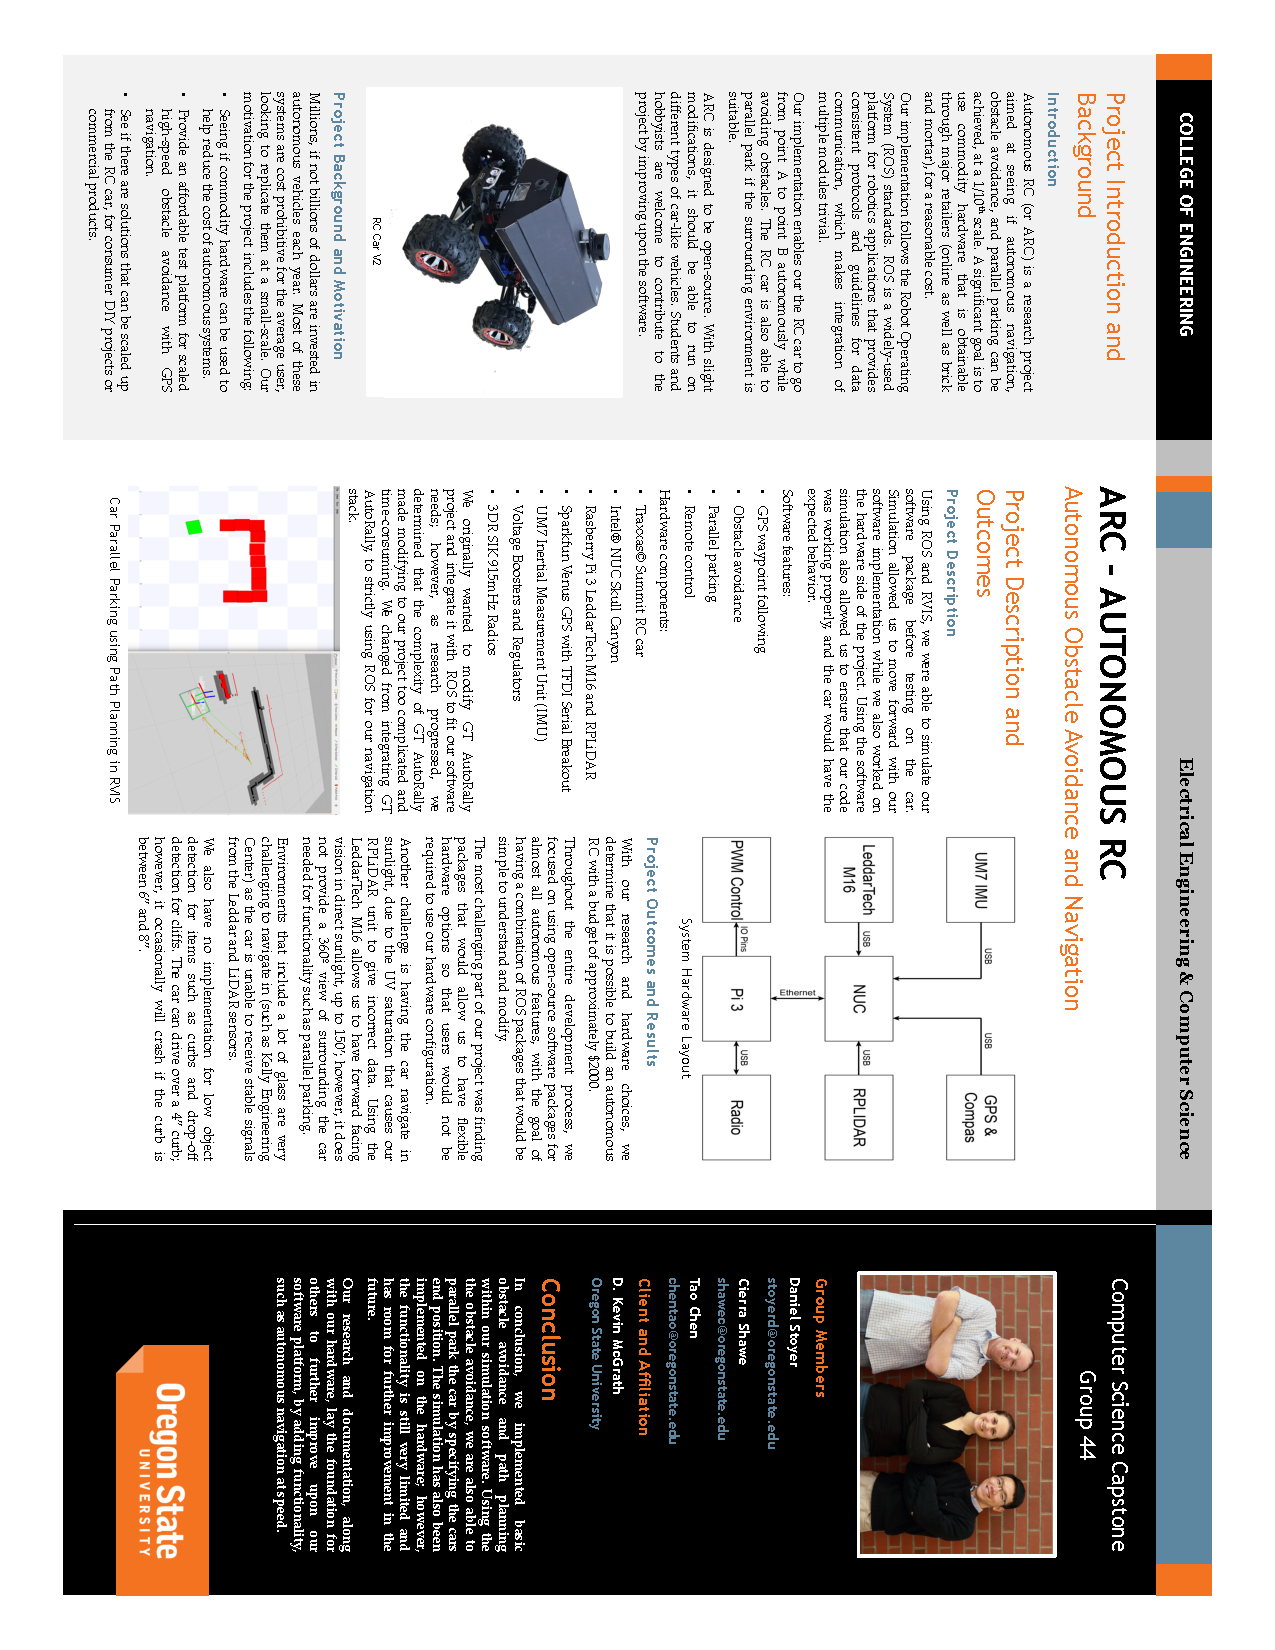
\includepdf[pages={-}]{project_poster.pdf}

\section{Project Documentation}
ARC is designed to be modular. We chose the Robotics Operating System as our primary software platform because it has a large number of libraries supporting many different types of sensors. You should be able to swap the sensors we chose (such as GPS, IMU, LiDAR units) with another of your choosing. Consider our parts list a minimum requirement for operation. More sensors (even duplicate sensors) can be added for greater accuracy in data.

\subsection{Structure}
The structure of ARC has two parts, software and hardware. The primary software platform is ROS Indigo. We also use Gazebo and Stage for simulation. We used AutoRally as a learning tool and provide instructions for how to install and use it. We moved away from AutoRally, but feel it is still a valuable tool to learn about vehicle simulation and ROS. Hardware-wise, we have a main computational unit that handles the heavy lifting for data collection and path-planning, a secondary computer for PWM control or autopilot communication (depending on which you go with), and GPS/IMU sensor integration.\\

% block diagram here
\begin{figure}[h]
    \centering
    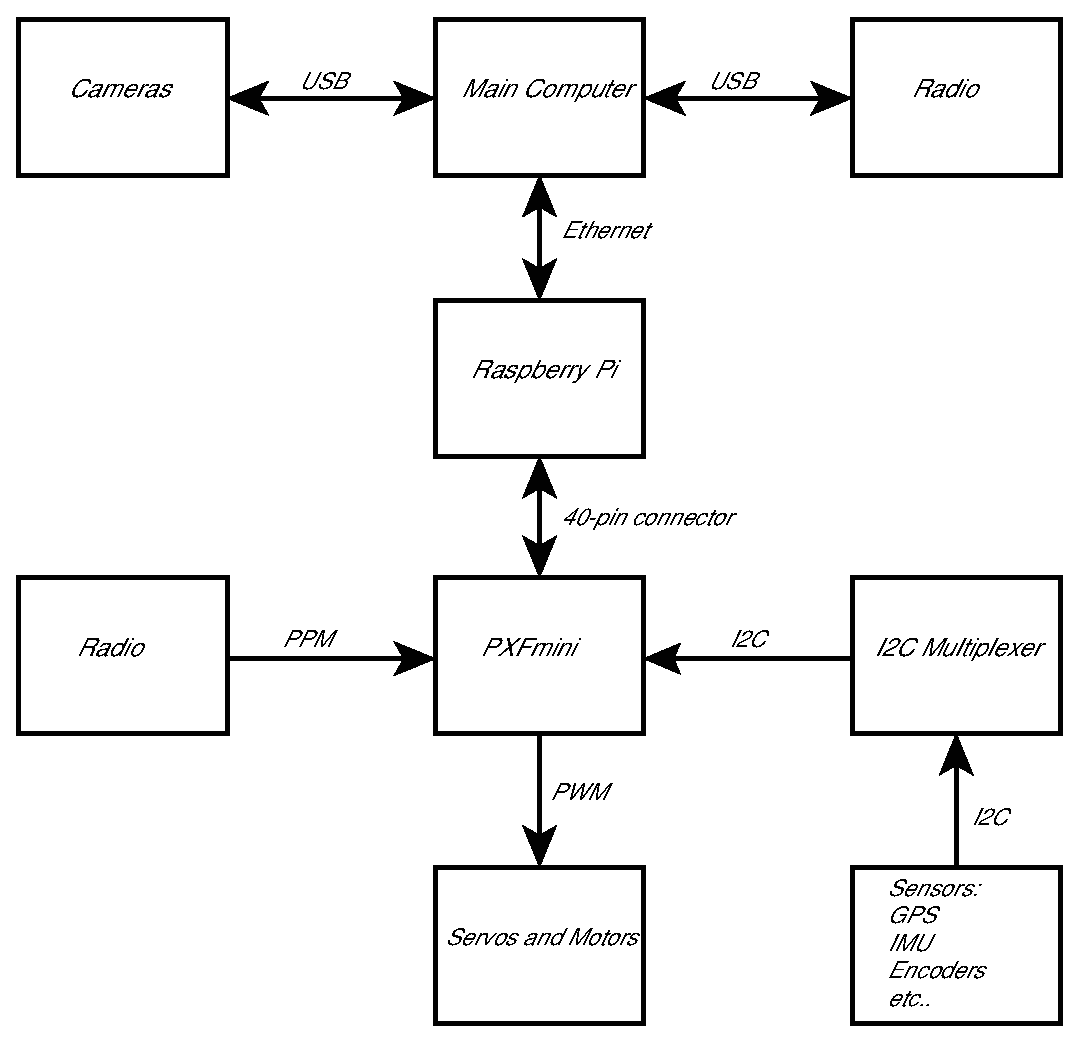
\includegraphics[scale=.5]{Block_Diagram}
    \caption{Main Project Components}
    \label{fig:my_label}
\end{figure}

\subsection{Software Installation}
\subsubsection{GT AutoRally Instructions}
Step-by-step instructions on how to run our implementation of the GT AutoRally simulation platform.
\begin{enumerate}
	\item Go to \href{https://github.com/AutoRally/autorally}{https://github.com/AutoRally/autorally} and follow the instructions to install the AutoRally platform. Be sure to follow the instructions carefully and completely, failure to do so may result in an incomplete installation that will require extended time to troubleshoot.\\
	NOTE: It is assumed from this point on that you have already gone
through the "Autonomous Driving in simulation" instructions at GT AutoRally.\\
	The following instructions are intended for after completing the GT AutoRally setup and simulation instructions above.
	\item At this point you should be able to run GT AutoRally
	\item Keep all simulation configuration according to the AutoRally specifications.\\ e.g. stateEstimator's InvertY and InvertZ values.
	\item Navigate to the work space where you put the AutoRally package. And then go to the src/autorally directory.
	NOTE: All files/folders modified and provided by ARC for AutoRally are found in the arc\_autorally folder.\\
	\item Under autorally\_description/urdf, replace the autoRallyPlatform.urdf.xacro file with file of the same name that we provide.
	\item Copy the world folder we provide to autorally\_description/models.
	\item Under autorally\_description, there is a file named empty\_sky\_AR.world. Copy the code below to the end of the file (before the last ""):\\ model://urdf/models/world
	\item Under autorally\_gazebo/launch, there is a file named autoRallyTrackWorld.launch, comment out the last node (named spawn\_track).
	\item Copy the autorally\_smartdriving folder to src/autorally.
	\item Open a terminal, navigate to your work space. The directory that contains devel/, src/ and build/.
	\item Use catkin\_make to compile the package.
	\item Open the bashrc by typing in gedit ~/.bashrc.
	\item At the bottom of the file, add these two lines: source workspace\_directory/devel/setup.bash source workspace\_directory/src/autorally/autorally\_util/setupEnvLocal.sh
	(Replace the workspace\_directory with your actually work space directory)
	\item Copy the run\_autorally.sh we provide to your work space.
	\item Open another terminal, navigate to your work space and run the run\_autorally.sh script.
	\item run\_autorally.sh script automates the initialization processes of the GT AutoRally simulation.
	\item A single terminal window opens opens with sub-divided windows using tmux.
	\item Applications necessary for AutoRally will open next, including Gazebo and rqt\_publisher. These applications along with other processes are launched by the script within different tmux sub-windows in the main terminal window.
	\item Find the application window (seperate from the terminal window) titled "rqt\_publisher".
	\item Go to rqt\_publisher and make sure the topics created during initial setup are still there:\\ /runStop /chassisState /constantSpeedController/speedCommand
	\item If rqt\_publisher does not have those three topics in the main part of the window, go back to the setup instructions and add them.
	\item Make sure /runStop is set to true and speed (under /speedCommand) is set to 3. Then check the boxes to the left of those three topics.
	\item Run these two commands in two of the tmux windows:\\ roslaunch autorally\_smartdriving autorally\_configuration.launch roslaunch autorally\_smartdriving move\_base.launch
	\item Go back to the rqt\_publisher window and uncheck the constantspeedcontroller message.
	\item Terminate the waypointfollower and the constantspeedcontroller.
	\item Copy the rviz config file we provide.
	\item roslaunch autorally\_smartdriving auto\_turn.launch
	\item run rviz with the rviz config file. rosrun rviz rviz
	\item Now you can set goals through Rviz and the car should go towards the goal autonomously.
\end{enumerate}


\subsubsection{ROS Indigo Installation}
If you are not installing AutoRally (which links you to the ROS installation instructions), then you will need to install ROS before doing anything else with ARC.\\
Go to \href{http://wiki.ros.org/indigo/Installation/Ubuntu}{http://wiki.ros.org/indigo/Installation/Ubuntu} and follow the official instructions for installing ROS Indigo.

 \subsubsection{Installing Sensor Packages}
ROS has pre-built packages for the sensors we used in this project. The instructions for installing those packages are below. If you use different sensors, you will need to install packages corresponding to your sensors, or write your own packages if none are available.
 \begin{itemize}
     \item SlamTech RPLiDAR
     \subitem - At the terminal command prompt:
     \subitem \$ sudo apt-get install ros-indigo-RPLiDAR-ros
     \item LeddarTech Evaluation Kit:
     \subitem - Go to the ROS-Leddar GitHub repository (\href{https://github.com/mcgill-robotics/ros-leddar}{https://github.com/mcgill-robotics/ros-leddar}, download (clone) the LeddarTech package and follow the instructions on that page.
     \item UM7 IMU:
     \subitem - At the terminal command prompt:
     \subitem \$ sudo apt-get install ros-indigo-um7
     \item Ublox GPS:
      \subitem - Clone the Ublox repository at       \href{https://github.com/KumarRobotics/ublox}{https://github.com/KumarRobotics/ublox} and floow the instructions on that page.
\end{itemize}

\subsubsection{Stage Installation Instructions}
All files modified by ARC for use in the Stage simulator are found in the arc\_stage folder provided.
\begin{enumerate}
    \item Extract the NewArc compressed file. In it there will be two packages named "smart driving" and "stage\_launch".
    \item Create a ROS work space, and copy the two packages to the src folder inside the new work space.
    \item On the root of the new work space, run "catkin\_make".
    \item On a new terminal, run "roscore".
    \item On the original terminal, run "source devel/setup.bash".
    \item On the original terminal, run "source devel/setup.bash".
    \item Run "roslaunch stage\_launch arc\_stage.launch".
    \item A stage simulator and Rviz should show up.
    \item The red blocks on the simulator can be moved around.
    \item Use the "2D Nav Goal" on Rviz to tell the car where to go.
\end{enumerate}


\subsection{Special Considerations}
\begin{itemize}
    \item Ubuntu 14.04 was used on the primary computer and is required for the version of ROS (Indigo) that we used.
    \item ARC requires use of ROS Indigo, specifically. Newer versions of ROS might work, but have not been tested.
    \item If you go with a PXFMini, you will need to get a custom Raspberry Pi 3 image from them.
\end{itemize}

\subsection{User Guides, API documentation, Etc.}
\begin{itemize}
    \item MAVLink API: \href{https://github.com/mavlink}{https://github.com/mavlink}
    \item Traxxas Summit owner's manual: \href{https://traxxas.com/sites/default/files/110829-R02-5607-manual.pdf}{https://traxxas.com/sites/default/files/110829-R02-5607-manual.pdf}
    \item PXFMini documentation: \href{http://docs.erlerobotics.com/brains/pxfmini}{http://docs.erlerobotics.com/brains/pxfmini}
\end{itemize}

\subsection{Parts List}
These are the final components we used for our vehicle. Note that all components in this list may be swapped out for different brands/technologies as long as the corresponding ROS packages are modified accordingly.\\
This list does not include all components we tested during research and development it is only the components on the final version of the RC car.


%FIXME item size
    \begin{table}[htbp]
    \resizebox{.75\textwidth}{!}{
    \begin{tabular}{|p{.66\textwidth}|p{.33\textwidth}|}

    %%%%%%%%%%%%%%%%%%%%%%%%%%%%%%%%%%%%
    %%% One row: %%%
    % Description w/URL (if necessary) &
    % Price &
    %%%%%
    % example:
    % Description
    % {\href{https://www.raspberrypi.org/products/raspberry-pi-3-model-b/}{Raspberry Pi 3}} &

    % Price
    % {\$45}
    % \hline
    %%%%%%%%%%%%%%%%%%%%%%%%%%%%%%%%%%%%
    \hline
    Description &
    Price \\
    \hline
    %%%%%%%%%%%%%%%%%%%%%%%%%%%%%%%%%%%%
    \hline
    Autopilot &
     \\
    \hline
    %%%%%%%%%%%%%%%%%%%%%%%%%%%%%%%%%%%%
    % Description
    {\href{https://www.raspberrypi.org/products/raspberry-pi-3-model-b/}{Raspberry Pi 3 (RPi3)}} &

    % Price
    {\$45}\\
    \hline
    %%%%%%%%%%%%%%%%%%%%%%%%%%%%%%%%%%%%
    % Description
    {\href{http://erlerobotics.com/blog/product/pxfmini/}{PXFmini}} &

    % Price
    {\$77.73}\\
    \hline
    %%%%%%%%%%%%%%%%%%%%%%%%%%%%%%%%%%%%
    OR &
     \\
    \hline
    %%%%%%%%%%%%%%%%%%%%%%%%%%%%%%%%%%%%
    % Description
    {\href{}{PWM Controller}} &

    % Price
    {\$3.95}\\
    \hline
    %%%%%%%%%%%%%%%%%%%%%%%%%%%%%%%%%%%%% Part Description
    % Description
    {\href{https://www.arduino.cc/}{Arduino}} &

    % Price
    {\$39.90}\\
    % extra \hline to separate the autopilot visually
    \hline
    \hline
    %%%%%%%%%%%%%%%%%%%%%%%%%%%%%%%%%%%%
    % Description
    {\href{https://www.u-blox.com/en/product/neo-m8-series}{Ublox Neo-M8N GPS with Compass}} &

    % Price
    {\$8.85}\\
    \hline
    %%%%%%%%%%%%%%%%%%%%%%%%%%%%%%%%%%%%
    % Description
    {\href{http://www.chrobotics.com/shop/um7-lt-orientation-sensor}{UM7-LT Orientation Sensor}} &

    % Price
    {\$139.95}\\
    \hline
    %%%%%%%%%%%%%%%%%%%%%%%%%%%%%%%%%%%%
    % Description
    {\href{https://3dr.com/wp-content/uploads/2017/03/3DR-Radio-V2-doc1.pdf}{3DR radios (2)}} &

    % Price
    {\$100.00}\\
    \hline
    %%%%%%%%%%%%%%%%%%%%%%%%%%%%%%%%%%%%
    % Description
    {\href{http://Leddartech.com/Leddar-evaluation-kit/}{LeddarTech Leddar Evaluation Kit}} &

    % Price
    {\$299.99}\\
    \hline
    %%%%%%%%%%%%%%%%%%%%%%%%%%%%%%%%%%%%
    % Description
    {\href{http://www.intel.com/content/www/us/en/nuc/nuc-kit-nuc6i7kyk-features-configurations.html}{Intel NUC Skull Canyon \newline With 16GB DDR4 and 480GB SSD}} &

    % Price
    {\$994.98}\\
    \hline
    %%%%%%%%%%%%%%%%%%%%%%%%%%%%%%%%%%%%
    % Description
    {\href{https://www.slamtec.com/en/LiDAR}{SlamTec RPLiDAR}} &

    % Price
    {\$199.00}\\
    \hline
    %%%%%%%%%%%%%%%%%%%%%%%%%%%%%%%%%%%
    % Description
    {Continued on next page.} &

    % Price
     \\
    \hline
    %%%%%%%%%%%%%%%%%%%%%%%%%%%%%%%%%%%

    \end{tabular}
    }
    \end{table}

    \begin{table}[htbp]
    \resizebox{.75\textwidth}{!}{
    \begin{tabular}{ |p{.66\textwidth}|p{.33\textwidth}|  }

    \hline
    % Description
    Component Sub-Totals &

    % Price
    \\
    \hline
    %%%%%%%%%%%%%%%%%%%%%%%%%%%%%%%%%%%
    % Description
    {Components with PXFMini/RPi3} &

    % Price
    {\textbf{\$1,865}}\\
    \hline
    %%%%%%%%%%%%%%%%%%%%%%%%%%%%%%%%%%%
    OR &
     \\
    \hline
    %%%%%%%%%%%%%%%%%%%%%%%%%%%%%%%%%%%
    % Description
    {Components with PWM/Arduino} &

    % Price
    {\textbf{\$1,785.63}}\\
    \hline
    %%%%%%%%%%%%%%%%%%%%%%%%%%%%%%%%%%%
    \hline
    % Description
    {\href{https://traxxas.com/products/models/electric/56076summit}{Traxxas Summit RC car}} &

    % Price
    {\$549.95}\\
    \hline
    \hline
    %%%%%%%%%%%%%%%%%%%%%%%%%%%%%%%%%%%
    Totals with RC car &

    % Price
    \\
    \hline
    %%%%%%%%%%%%%%%%%%%%%%%%%%%%%%%%%%%
    % Description
    {Using PXFMini/RPi3} &

    % Price
    {\textbf{\$2,414.46}}\\
    \hline
    %%%%%%%%%%%%%%%%%%%%%%%%%%%%%%%%%%%
    OR &
     \\
    \hline
    %%%%%%%%%%%%%%%%%%%%%%%%%%%%%%%%%%%
    % Description
    {Using PWM/Arduino} &

    % Price
    {\textbf{\$2,335.58}}\\
    \hline
    %%%%%%%%%%%%%%%%%%%%%%%%%%%%%%%%%%%

    \end{tabular}
    }
    \end{table}





\section{New Technology Learned}
%FIXME There is a lot more to this than just ROS and two websites...
As a whole, every piece of technology we touched within the project was new to us, which was one of the hardest parts of the project.

\textit{What web sites were helpful?}
\begin{itemize}
    \item \url{http://wiki.ros.org}\par
        The ROS wiki provides documentations and tutorials on packages.\par
        A documentation of a specific package includes:
        \begin{itemize}
            \item Compatibility to different versions of ROS.
            \item Package version and release status.
            \item The github repository where all the source code is stored.
            \item Installation and setup guide.
            \item Prototypes of APIs and detailed descriptions of the APIs.
            \item Detailed descriptions of parameters that can be used to configure the package.
        \end{itemize}
         A tutorial of a specific package includes:
        \begin{itemize}
            \item Introduction to the package.
            \item Different scenarios where the package can be used.
            \item Detailed walk-through of implementation of each scenario.
        \end{itemize}
    \item \url{http://docs.ros.org}\par
        The ROS doc has detailed descriptions of data types that messages must obey for nodes to send and receive. This is extremely useful because even though ROS uses C++ and Python, it has a large number of customized data types. We had to configure our nodes correctly to publish and subscribe messages, so that the nodes can communicate and modules can be integrated.
    \item \url{https://github.com/AutoRally/autorally}\par
        At the beginning of this project, we referred to the AutoRally project a lot to look for ideas. The project is entirely open-source, which means all the code is in the repository. There is step-by-step guides on how to set up the platform and detailed descriptions of individual components. The repository also had a breakdown list of parts (hardware) the platform used. It was the configuration to which we compared our platform, both cost-wise and power-wise.
\end{itemize}

\textit{Reference Books}

\textit{Helper People}


\section{What We Learned}
%FIXME THIS IS NOT SUPPOSED TO BE A LIST, it needs to be reformatted into paragraph formatting.

We experienced how a research project was approximately carried out.

We got to work in a diverse team, which helped us improve our communication skills.

When working in a small team, the relationship between teammates became more intimate, which make us become more considerate people.

We learned a lot on how to use ROS.

ROS was a big part of this project, and we only had little to no experience working with it.

What we were able to accomplish was incredible.

MORE TO ADD.


\subsection{Cierra}
\subsubsection*{What technical information did you learn?}

\textit{Reading technical specifications for a product:\\}
The first time I tried to read a product specification document, I had no idea how to even find information about it.
Being able to read these types of documents was incredibly important throughout the project, as I needed to see how were were supposed to wire all of our components together.

\textit{Reading a wiring diagram:\\}
This was really important, as many of the things we were given did not have headers or ways of attaching the wires to our other components.
While someone from ECE might think it was a trivial task, it took a little while to understand what the different things meant.

\textit{Working with ROS:\\}
Unlike the rest of my group, I did not have quite as much exposure to ROS throughout the project, as I ended up taking a primarily hardware role.
I did learn the basics of how it is used through the tutorial and through my teammates. I hope to be able to spend more time learning the details of ROS, as it definitely is a useful tool for robotics, as most things are already implemented for you.

\textit{Soldering:\\}
The only thing I had ever soldered in my life before this project was a little light-up pin one day at the fair.
While the idea is simple, I learned a lot about how to properly splice wires, how to de-solder (and how you want to avoid this at all costs), and how to ensure soldered components will not easily come loose. I also gained a lot of respect for the ECE students, as it is really hard to make a clean looking board.

\textit{Voltage conversion (and how to not fry components):\\}
This was incredibly important, as a lot of our components required odd voltages. In order to convert from 12V to whatever else we needed, I used voltage boosters to be able to use the NUC and leddar at 19V and 24V respectively. I also learned that separating components (such as the PWM board) on to their own power system is important, as we kept dropping the Arduino and Raspberry Pi too low, so they should shut down. With each component we added, I always made sure to read the specifications of what it needed, and then ensured that it was being provided the correct voltage and current with a voltmeter. I also learned just because something says it can take either 12V or 24V, does not mean it can take both, it means that somewhere on the poorly documented board, there could be a jumper that allows you to change from 12-24v. Providing something 12V that is looking for 24V, could lead to it frying the component. This is in reference to our Leddar, which we still do not know why it broke.

\textit{How to control servos and motors with a Raspberry Pi and Arduino:\\}
While both the Arduino and Raspberry Pi are able to directly control servos, it was a lot easier to use a motor control board. One thing I noticed, is that the was considerable lag in the system when the Arduino or Raspberry Pi power dropped too low.

\textit{Working with LiDAR systems:\\}
Before the project, I had never actually see a point cloud created before. Now I have a much stronger understanding and appreciation for LiDAR devices, as they can do some pretty incredible things. The cool part about using ROS, is all of these implementations became trivial, as it is a built in feature of a "LaserScan" topic.

\subsubsection*{What non-technical information did you learn?}
I have always struggled with trying to explain my thoughts and ideas, especially through writing.
Before this year, writing papers always seemed dreadful.
As much as I disliked the WIC inclusion into Capstone, I feel it has improved my ability to create documents and critically think about a problem before starting.
It is incredibly satisfying to be able to sit down and write a paper, without it taking a million years.
I am now able to break down a problem into more manageable pieces, instead of being overwhelmed by everything at once.
Also, ten pages seems like a trivial amount of work now, which has made all of my other classes a lot easier when we had to write various project reports. \par


\subsubsection*{What have you learned about project work?}
Planning is essential if you expect a project to go well. I would say as a whole we did a really good job creating good guidelines, but we fell short in estimating and having back up plans for when we found out things just would not work.

Being able to track tasks with some sort of management software would have been nice as well. We had tried to start using an agile method fall term, but it was really difficult considering everyone was also having to juggle their other classes and there were not a lot of times we could sit down and get together to break things into specific tasks. Instead, a lot of the task breakdown was done by hangouts, which often made it difficult to go back and figure out who was responsible for what parts of a paper or the project.

\subsubsection*{What have you learned about project management?}
Of of the biggest things I learned, was always assume things will take more time than what you originally expect. Our biggest setback was not having allocated enough time in the beginning. As I was the one who submitted the majority of our work, I also learned that plenty of time should be left around a deadline to account for potential problems that may occur.

Communication is also key, and I feel like I am able to take a step back and say "This is what we need to do, now how are we going to get there?" Since at the beginning of the project, we had no experience with anything we were going to be using, stepping back and trying to break the problem down into smaller pieces was key.

\subsubsection*{What have you learned about working in teams?}
Communication is incredibly important. Take a step back and make sure everyone is on the same page before moving onto a different task.

\subsubsection*{If you could do it all over, what would you do differently?}
If I could start over, I would have made sure to not get hung up on something for too long. If we had been able to accept that the PXFmini was not going to work for our situation, we would have been able to start implementing things earlier in the term.
Finally, I would take any time estimates and quadruple them. Nothing will go as planned, so you need to be able to adapt to whatever is thrown your way.


\subsection{Tao}

\subsubsection*{What technical information did you learn?}
\begin{itemize}
    \item A basic structure of a project.
    \item Using ROS.
    \item Version control.
\end{itemize}

\subsubsection*{What non-technical information did you learn?}
\begin{itemize}
    \item Communicating with teammates.
    \item Explaining concepts and reporting to client.
    \item Recording progress.
    \item For me personally, this project made me like to think about
    problems with the big picture while focusing on the individual components.
\end{itemize}

\subsubsection*{What have you learned about project work?}
\begin{itemize}
    \item Coding could be easy if the project was planed out nicely.
    \item To make a good plan, one must view the project from different
    perspectives, and listen to others' opinions.
    \item Keeping track of progress is extremely important.
    \item Stick with the plan, and yet quickly switch other solutions
    when the original does not work out.
\end{itemize}

\subsubsection*{What have you learned about project management?}
\begin{itemize}
    \item Lists are useful for keeping track of hardware.
    \item Version control is important but be careful when using it.
\end{itemize}

\subsubsection*{What have you learned about working in teams?}
\begin{itemize}
    \item Good teammates are key. It depends on luck.
    \item Always try to create a positive atmosphere even things aren't
    working so well.
    \item Helping teammates out is not sacrificing. You gain more than you
    lose.
\end{itemize}

\subsubsection*{If you could do it all over, what would you do differently?}
\begin{itemize}
  \item I'd probably prioritize things differently and look for other options
  when something didn't work out. For example, we could have worked on the
  software and hardware simultaneously, which I think was our original plan.
  But then we hit a road block that totally stalled our work on hardware from
  progressing. Other than that, I don't think I would do much different.
\end{itemize}


\subsection{Dan}
\subsubsection*{What technical information did you learn?}
\begin{itemize}
    \item How to develop for robots:\\
    The Robotics Operating System (ROS) is an open source general-purpose software
    platform for developers working with all manner of robots. ROS allows the developer to
    use its extensive libraries to implement custom code for controlling robots and provides communications and navigation libraries that are very useful for autonomous vehicle applications. We wrote some programs in C and python using Ros libraries to communicate with the vehicle.
    \item How to set up simulators:\\
    I used both Gazebo and Stage are simulation environments that we used on this project. I learned how to set up and run both.
    \item RC cars and Autonomy\\
    I had never worked with RC cars, or tried any sort of robotics, so diving into the field of autonomous vehicles really stretched me. There is \textit{so much} that goes into research and development of autonomous vehicles. The computer has to either know the exact state of the vehicle via sensor data, or be able to estimate the vehicle's state closely enough to operate.
    \item \href{https:\\cmake.org}{CMake}\\
    CMake is a platform for build and testing software. It is open source. ROS uses CMake as part of its package installation platform, called Catkin.
    \item I learned more about bash and Linux, creating a script to launch AutoRally, spawning multiple terminals and processes.
    \item I learned about LiDAR and point-clouds. I had never seen LiDAR in action before. I learned that there are different types of LiDAR. We used IR and some sort of LED technology.
\end{itemize}

\subsubsection*{What non-technical information did you learn?}
\begin{itemize}
    \item I learned that "autonomous" has many different meanings when related to vehicles. My assumption was that it meant that cars could navigate pretty much anywhere on their own. I found out that a car can be considered "autonomous" if it performs \textit{any} operation on its own. For instance, Georgia Tech's AutoRally project claims their car is "autonomous" and the car does go around a track without a user controlling the car directly. However, the car does guide itself, it follows predetermined way-points and performs no obstacle avoidance what-so-ever. The barriers around the track were in place to merely keep the car from going completely off the rails should something go wrong. The car did self-correct steering around the turns and kept the car under control will power-sliding around corners. So, the car was autonomous, just not in the way that I had though.
\end{itemize}

\subsubsection*{What have you learned about project work?}
\begin{itemize}
\item Plan for setbacks and do not be disappointed when they happen.
    \item It's really hard to work on a complicated project part time while taking other classes.
    \item Ten hours of trial and error will save an hour of good design planning.
\end{itemize}

\subsubsection*{ What have you learned about project management?}
\begin{itemize}
    \item It would be very helpful to use project management software.
    \subitem My team did \textit{not} use any sort of project management software for this project, by "project management software" I mean packages such as MS Project, or Redmine. Project tracking using manually implemented Gantt charts was incredibly tedious and not really used as a practical tool.
    \item Milestones need to be clearly identified and consistently communicated throughout the life of the project.
\end{itemize}

\subsubsection*{What have you learned about working in teams?}
\begin{itemize}
    \item I was the team leader. It was difficult to balance keeping the team focused on our goal and not squashing enthusiasm when attempting to redirect tangent ideas back on track.
    \item Good communication is key to keeping a team operating smoothly.
    \item When everyone pitches in and they are enthusiastic about the project, the work is quite fun.
\end{itemize}

\subsubsection*{If you could do it all over, what would you do differently?}
\begin{itemize}
    \item Identify critical points of failure. Things that could possibly set us back significantly if they were to fail.
    \subitem Test those points early, if possible.
    \item Be more proactive about getting help for problems. Don't struggle with a problem for more than a few days before getting help.
    \item Start with a rover that has an autopilot integrated into it, possibly even already has some sensors on it.
    \subitem Our team had \textit{no} experience going into this project. Trying to start from scratch was probably a bit too much, if the goal was to implement high-speed performance. It would have been more realistic to attain if we had started with a vehicle that had some sort of autonomous capability already and then we "upgrade" it to perform at a high rate of speed.
    \item I would use project management software.
    \item I would set an expectation of a required weekly meeting time at the beginning of the project. Our team agreed to do that, but I did not really follow through on it well.
\end{itemize}


\section{ARC Findings and Conclusions}
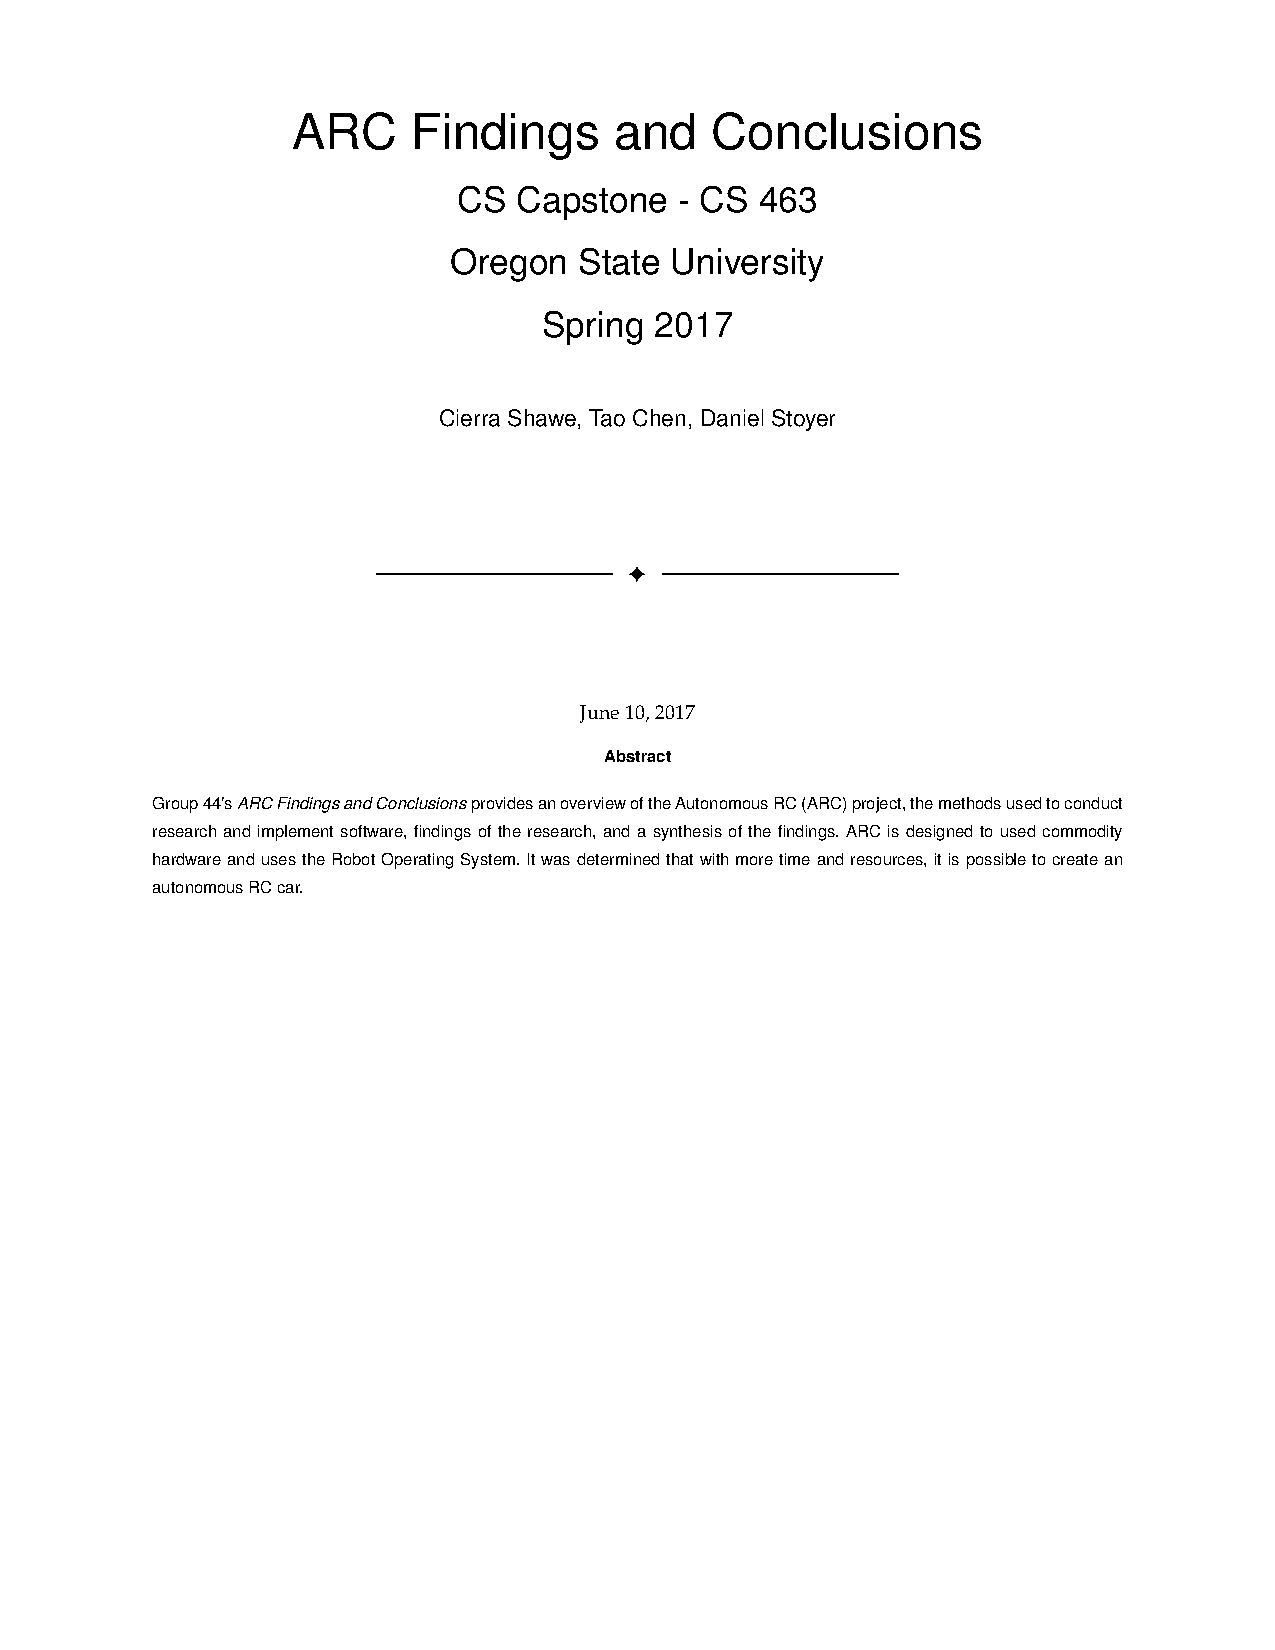
\includepdf[pages={-}]{write_up.pdf}

\section{Appendix 1}
Essential Code Listings. You don't have to include absolutely everything, but if someone wants to understand your project, there should be enough here to learn from. If you worked within a larger project, something like a patch file might be a good way to go.
\begin{lstlisting}[frame=single,caption={Example Custom ROS Node}]
/**********************************************
* @file LiDARDetection.cpp
* @author Tao Chen <chentao@oregonstate.edu>
* @date Feburary 21, 2017
* @copyright 2017 Oregon State University
* @brief ROS node to generate new waypoints based on LiDAR scan
*
* @details When an obstacle is detected, it alters the original
* set of waypoints to go around the obstacle. This node subscribes to
* the laser_scan message and the current_list_of_waypoints message and
* publish the new_waypoints message.
***********************************************/

#include "LiDARDetection.h"

namespace autorally_smartdriving{
	LiDARDetection::LiDARDetection(){
		l_LiDARSub = l_nh.subscribe("/autorally_platform/laser_scan", 10, &LiDARDetection::gatherLiDARData, this);
		l_LiDARPub = l_nh.advertise<sensor_msgs::LaserScan>("scan", 10);

		samples = 2000;
		laser_frequency = 10;
		scan.ranges.resize(samples);
		scan.intensities.resize(samples);
	}

	LiDARDetection::~LiDARDetection(){}

	void LiDARDetection::gatherLiDARData(sensor_msgs::LaserScan data){
		int counter = 0;

		ros::Time scan_time = ros::Time::now();

		scan.header.stamp = scan_time;
		scan.header.frame_id = "LiDAR";
		scan.angle_min = data.angle_min;
		scan.angle_max = data.angle_max;
		scan.angle_increment = data.angle_max / samples;
		scan.time_increment = (1 / laser_frequency) / samples;
		scan.range_min = data.range_min;
		scan.range_max = data.range_max;

		for(counter = 0; counter < samples; counter++){
			scan.ranges[counter] = data.ranges[counter];
			scan.intensities[counter] = data.intensities[counter];
		}

		// publish scan to scan topic
		l_LiDARPub.publish(scan);
	}
};

int main(int argc, char** argv){
	ros::init(argc, argv, "LiDARDetection");
	autorally_smartdriving::LiDARDetection LiDARDetection;
	ros::spin();
}
\end{lstlisting}

\begin{lstlisting}[frame=single,caption={Example Custom Launch File for Stage}]
<launch>

  <!--  ************** Global Parameters ***************  -->
  <param name="/use_sim_time" value="true"/>

  <!--  ************** Stage simulator ***************  -->
  <node pkg="stage_ros" type="stageros" name="stageros" args="$(find stage_launch)/stage/empty.world">
    <!-- <remap from="base_scan" to="scan"/> -->
    <remap from="base_scan" to="base_scan_0"/>
  </node>

  <node pkg="move_base" type="move_base" respawn="false" name="move_base" output="screen">
    <rosparam file="$(find smart_driving)/config/costmap_common_params.yaml" command="load" ns="global_costmap" />
    <rosparam file="$(find smart_driving)/config/costmap_common_params.yaml" command="load" ns="local_costmap" />
    <rosparam file="$(find smart_driving)/config/local_costmap_params.yaml" command="load" />
    <rosparam file="$(find smart_driving)/config/global_costmap_params.yaml" command="load" />
    <rosparam file="$(find smart_driving)/config/base_local_planner_params.yaml" command="load" />

    <param name="base_global_planner" value="global_planner/GlobalPlanner" />
    <param name="planner_frequency" value="1.0" />
    <param name="planner_patience" value="5.0" />

    <param name="base_local_planner" value="teb_local_planner/TebLocalPlannerROS" />
    <param name="controller_frequency" value="5.0" />
    <param name="controller_patience" value="15.0" />

    <param name="clearing_rotation_allowed" value="false" />
  </node>

  <node name="map_server" pkg="map_server" type="map_server" args="$(find stage_launch)/maps/empty_world.yaml" output="screen">
    <param name="frame_id" value="/map" />
  </node>

  <!--<node pkg="amcl" type="amcl" name="amcl" output="screen">
    <rosparam file="$(find stage_launch)/cfg/amcl_params.yaml" command="load"/>
    <param name="initial_pose_x" value="0" />
    <param name="initial_pose_y" value="0" />
    <param name="initial_pose_z" value="0" />
  </ode>-->

  <!-- <include file="$(find Leddar)/launch/Leddar.launch">
    <arg name="serial" value="AJ04071" />
    <arg name="frame" value="base_laser_link_0" />
    <arg name="fov" value="45" />
    <arg name="range" value="50" />
  </include> -->

  <include file="$(find stage_launch)/robot_localization.launch"/>

  <node name="odom" pkg="autorally_smartdriving" type="odom" />
  <node name="rviz" pkg="rviz" type="rviz" args="-d $(find stage_launch)/stage/rviz_navigation.rviz"/>
</launch>
\end{lstlisting}

\begin{lstlisting}[frame=single,caption={ROS odom/transform node (not including the .h file.
The .h file is located in our github repository)}]
/**********************************************
* @file odom.cpp
* @author Tao Chen <chentao@oregonstate.edu>
* @date Feburary 25, 2017
* @copyright 2017 Oregon State University
* @brief pulishes odometry data to the navigation stack
*
* @details This node subscribes to odometry data from /autorally_platform
and publisher the data to the navigation stack
***********************************************/

#include "odom.h"

namespace autorally_smartdriving{
  Odom::Odom(){
    o_odomSub = o_nh.subscribe("/base_pose_ground_truth", 1, &Odom::gatherOdomData, this);
    o_odomPub = o_nh.advertise<nav_msgs::Odometry>("odom", 1);
    o_PoseArrayPub = o_nh.advertise<geometry_msgs::PoseArray>("particlecloud", 1);
    o_poseCovariancePub = o_nh.advertise<geometry_msgs::PoseWithCovarianceStamped>("amcl_pose", 1);
  }

  Odom::~Odom(){};

  void Odom::gatherOdomData(nav_msgs::Odometry data){
    tf::TransformBroadcaster odom_broadcaster;
    ros::Time time_stamp = ros::Time::now();

    //publish transform over tf
    geometry_msgs::TransformStamped odom_trans;
    geometry_msgs::TransformStamped map_trans;

    odom_trans.header.stamp = time_stamp;
    odom_trans.header.frame_id = "odom";             //base_link
    odom_trans.child_frame_id = "base_footprint";     //odom

    odom_trans.transform.translation.x = 0;
    odom_trans.transform.translation.y = 0;
    odom_trans.transform.translation.z = 0;
    odom_trans.transform.rotation.x = 0;
    odom_trans.transform.rotation.y = 0;
    odom_trans.transform.rotation.z = 0;
    odom_trans.transform.rotation.w = 1;

    /*odom_trans.transform.rotation.x = data.pose.pose.orientation.x;
    odom_trans.transform.rotation.y = data.pose.pose.orientation.y;
    odom_trans.transform.rotation.z = data.pose.pose.orientation.z;
    odom_trans.transform.rotation.w = data.pose.pose.orientation.w;*/

    map_trans.header.stamp = time_stamp;
    map_trans.header.frame_id = "map";
    map_trans.child_frame_id = "odom";        //base_link

    map_trans.transform.translation.x = data.pose.pose.position.x;
    map_trans.transform.translation.y = data.pose.pose.position.y;
    map_trans.transform.translation.z = data.pose.pose.position.z;
    map_trans.transform.rotation.x = data.pose.pose.orientation.x;
    map_trans.transform.rotation.y = data.pose.pose.orientation.y;
    map_trans.transform.rotation.z = data.pose.pose.orientation.z;
    map_trans.transform.rotation.w = data.pose.pose.orientation.w;

    /*map_trans.transform.rotation.x = 0;
    map_trans.transform.rotation.y = 0;
    map_trans.transform.rotation.z = 0;
    map_trans.transform.rotation.w = -1;*/

    //send the transform
    odom_broadcaster.sendTransform(odom_trans);
    odom_broadcaster.sendTransform(map_trans);

    //Publish pose array
    geometry_msgs::PoseArray poseArray;
    poseArray.poses.resize(1);
    poseArray.header.stamp = time_stamp;
    poseArray.header.frame_id = "map";

    for(int i = 0; i < 1; i++){
      poseArray.poses[i].position.x = data.pose.pose.position.x;
      poseArray.poses[i].position.y = data.pose.pose.position.y;
      poseArray.poses[i].position.z = data.pose.pose.position.z;

      poseArray.poses[i].orientation.x = data.pose.pose.orientation.x;
      poseArray.poses[i].orientation.y = data.pose.pose.orientation.y;
      poseArray.poses[i].orientation.z = data.pose.pose.orientation.z;
      poseArray.poses[i].orientation.w = data.pose.pose.orientation.w;
    }
    o_PoseArrayPub.publish(poseArray);

    //Publish pose with covariance
    geometry_msgs::PoseWithCovarianceStamped PoseWithCovariance;
    PoseWithCovariance.header.stamp = time_stamp;
    PoseWithCovariance.header.frame_id = "map";
    PoseWithCovariance.pose.pose.position.x = data.pose.pose.position.x;
    PoseWithCovariance.pose.pose.position.y = data.pose.pose.position.y;
    PoseWithCovariance.pose.pose.position.z = data.pose.pose.position.z;

    PoseWithCovariance.pose.covariance = data.pose.covariance;
    o_poseCovariancePub.publish(PoseWithCovariance);

    //add frame_id and child_frame to odom message
    data.header.stamp = time_stamp;
    data.header.frame_id = "map";

    data.child_frame_id = "odom";
    o_odomPub.publish(data);
  }
};

int main(int argc, char** argv){
  ros::init(argc, argv, "OdomNav");
  autorally_smartdriving::Odom odom;
  ros::spin();
}
\end{lstlisting}

\begin{lstlisting}[frame=single,caption={Example launch file}]
<launch>
  <include file="$(find autorally_core)/launch/hardware.machine" />
  <!-- Run the map server -->
  <node name="map_server" pkg="map_server" type="map_server" args="$(find autorally_smartdriving)/launch/test_map_empty.yaml"/>

  <node pkg="move_base" type="move_base" respawn="false" name="move_base" output="screen">
    <rosparam file="$(find autorally_smartdriving)/config/costmap_common_params.yaml" command="load" ns="global_costmap" />
    <rosparam file="$(find autorally_smartdriving)/config/costmap_common_params.yaml" command="load" ns="local_costmap" />
    <rosparam file="$(find autorally_smartdriving)/config/local_costmap_params.yaml" command="load" />
    <rosparam file="$(find autorally_smartdriving)/config/global_costmap_params.yaml" command="load" />
    <rosparam file="$(find autorally_smartdriving)/config/base_local_planner_params.yaml" command="load" />

    <param name="base_global_planner" value="global_planner/GlobalPlanner" />
    <param name="planner_frequency" value="1.0" />
    <param name="planner_patience" value="5.0" />

    <param name="base_local_planner" value="teb_local_planner/TebLocalPlannerROS" />
    <param name="controller_frequency" value="5.0" />
    <param name="controller_patience" value="15.0" />

    <param name="clearing_rotation_allowed" value="false" /> <!-- our vehicle can't rotate inplace -->
  </node>
</launch>
\end{lstlisting}

\begin{lstlisting}[frame=single,caption={Example package config file}]
<?xml version="1.0"?>
<package>
  <name>autorally_smartdriving</name>
  <version>0.0.0</version>
  <description>This package contains all the necessary files to enable the car to detect and avoid obstacle using the teb_local_planner package.</description>

  <maintainer email="chentao@oregonstate.edu">Tao Chen</maintainer>

  <license>BSD</license>

  <url type="website">https://github.com/cshawe/cs46x</url>

  <author email="chentao@oregonstate.edu">Tao Chen</author>

  <buildtool_depend>catkin</buildtool_depend>

  <build_depend>roscpp</build_depend>
  <build_depend>rospy</build_depend>
  <build_depend>std_msgs</build_depend>
  <build_depend>tf</build_depend>
  <build_depend>nodelet</build_depend>
  <build_depend>sensor_msgs</build_depend>
  <build_depend>geometry_msgs</build_depend>
  <build_depend>nav_msgs</build_depend>
  <build_depend>autorally_msgs</build_depend>
  <build_depend>move_base</build_depend>
  <build_depend>my_odom_configuration_dep</build_depend>
  <build_depend>my_sensor_configuration_dep</build_depend>
  <build_depend>my_tf_configuration_dep</build_depend>

  <run_depend>roscpp</run_depend>
  <run_depend>rospy</run_depend>
  <run_depend>std_msgs</run_depend>
  <run_depend>tf</run_depend>
  <run_depend>nodelet</run_depend>
  <run_depend>sensor_msgs</run_depend>
  <run_depend>geometry_msgs</run_depend>
  <run_depend>nav_msgs</run_depend>
  <run_depend>autorally_msgs</run_depend>
  <run_depend>move_base</run_depend>
  <run_depend>my_odom_configuration_dep</run_depend>
  <run_depend>my_sensor_configuration_dep</run_depend>
  <run_depend>my_tf_configuration_dep</run_depend>


  <!-- The export tag contains other, unspecified, tags -->
  <export>
    <!-- Other tools can request additional information be placed here -->

  </export>
</package>
\end{lstlisting}

\begin{lstlisting}[frame=single,caption={Example yaml (package params) file}]
# footprint is like the shadow of the vehicle if the light is shining from directly above.
# Assume that the center of the vehicle is (0, 0)
footprint: [[-0.3, 0.15], [0.3, 0.15], [0.3, -0.15], [-0.3, -0.15]]

transform_tolerance: 0.5      # undecided
map_type: costmap

obstacle_layer:
  enabled: true
  # MaxIMUm range sensor reading that will result in an obstacle being put into the costmap
  # 8.0 means the robot will only updata its map with info about obstacles that are within
  # 8.0 meters of the base.
  obstacle_range: 8.0
  # 5.0 means that the robot will attemp to clear out space in front of it up to 5.0 meters
  # away given sensor reading.
  raytrace_range: 5.0
  # This value determines how far the vehicle will stay away from obstacles.
  inflation_radius: 1.0
  # from the tutorial
  track_unknown_space: false
  combination_method: 1
  # we are only using laser scan
  observation_sources: laser_scan_sensor
  # marking and clearing mean that the sensor data will be used to mark and clear obstacle info
  # on the costmap
  laser_scan_sensor: {sensor_frame: LiDAR, data_type: LaserScan, topic: scan, marking: true, clearing: true, expected_update_rate: 0.5}

inflation_layer:
  enabled: true
  cost_scaling_factor: 10.0   # exponential rate at which the obstacle cost drops off
  inflation_radius: 1.0      # max distance from an obstacle at which costs are incurred for planning paths.

static_layer:
  enabled: true
map_topic: "/map"
\end{lstlisting}

\begin{lstlisting}[frame=single,caption={Example cmakelist file}]
cmake_minIMUm_required(VERSION 2.8.3)
project(autorally_smartdriving)

find_package(catkin REQUIRED COMPONENTS
  roscpp
  rospy
  std_msgs
  sensor_msgs
  geometry_msgs
  nav_msgs
  tf
)

catkin_package(
  INCLUDE_DIRS include
)

include_directories(
  include ${catkin_INCLUDE_DIRS}
)

add_subdirectory(src/LiDARDetection)
add_subdirectory(src/Odom)
add_subdirectory(src/Global_Path)
add_subdirectory(src/Drive)
add_subdirectory(src/IMU)

install(DIRECTORY launch/
   DESTINATION ${CATKIN_PACKAGE_SHARE_DESTINATION}/launch
   FILES_MATCHING PATTERN "*.launch" PATTERN "*.machine"
)

install(DIRECTORY include/${PROJECT_NAME}/
   DESTINATION ${CATKIN_PACKAGE_INCLUDE_DESTINATION}
)

install(DIRECTORY cfg/cpp/${PROJECT_NAME}/
   DESTINATION ${CATKIN_PACKAGE_INCLUDE_DESTINATION}
   FILES_MATCHING PATTERN "*.h"
)
\end{lstlisting}

\begin{lstlisting}[frame=single,caption={Example stage config file}]
include "arc_robot.inc"
include "block.inc"


define floorplan model
(
  # sombre, sensible, artistic
  color "gray30"

  # most maps will need a bounding box
  boundary 1

  gui_nose 0
  gui_grid 0
  gui_outline 0
  gripper_return 0
  fiducial_return 0
  laser_return 1
)

resolution 0.02
interval_sim 100  # simulation timestep in milliseconds

window
(
  size [ 600.0 700.0 ]
  center [ 0.0 0.0 ]
  rotate [ 0.0 0.0 ]
  scale 60
)

floorplan
(
  name "empty_world"
  bitmap "../maps/empty_world.png"
  size [ 200.0 200.0 2.0 ]
  pose [ 0.0 0.0 0.0 0.0 ]
)

# throw in a robot
carlike_robot
(
  pose [ 0.0 0.0 0.0 0.0 ]
  name "robot"
)

# adding blocks
block ( pose [2.0 4.0 0.0 0.0] color "red")
block ( pose [4.0 4.0 0.0 0.0] color "red")
block ( pose [6.0 4.0 0.0 0.0] color "red")
block ( pose [8.0 4.0 0.0 0.0] color "red")
block ( pose [10.0 4.0 0.0 0.0] color "red")
block ( pose [12.0 4.0 0.0 0.0] color "red")
block ( pose [14.0 4.0 0.0 0.0] color "red")
block ( pose [16.0 4.0 0.0 0.0] color "red")
block ( pose [18.0 4.0 0.0 0.0] color "red")
block ( pose [20.0 4.0 0.0 0.0] color "red")
block ( pose [22.0 4.0 0.0 0.0] color "red")
\end{lstlisting}

\begin{lstlisting}[frame=single,caption={Car description for stage}]
define laser ranger
(
  sensor
  (
    range_max 6
    fov 360
    samples 2000
  )

  color "black"
  size [ 0.06 0.15 0.03]
)

define Leddar ranger
(
  sensor
  (
    range_max 50.0
    fov 45
    samples 16
  )
  color "black"
  size [0.06 0.15 0.03]
)

define carlike_robot position
(
  pose [ 0.0 0.0 0.0 0.0 ]

  odom_error [ 0.03 0.03 999999 999999 999999 0.02 ]

  size [ 0.56 0.46 0.4 ]
  origin [ 0.2 0.0 0.0 0.0]
  gui_nose 1
  color "green"

  drive "car"
  localization "gps"
  wheelbase 0.38

  #laser(pose [-0.1 0.0 -0.11 0.0])
  laser(pose [0.1 0.0 -0.11 0.0])

  Leddar(pose [0.2 0.0 -0.11 0.0])
)
\end{lstlisting}

\section{Appendix 2}
Anything else you want to include. Photos, etc.

\end{document}
